% Created by tikzDevice version 0.7.0 on 2014-06-30 20:14:14
% !TEX encoding = UTF-8 Unicode
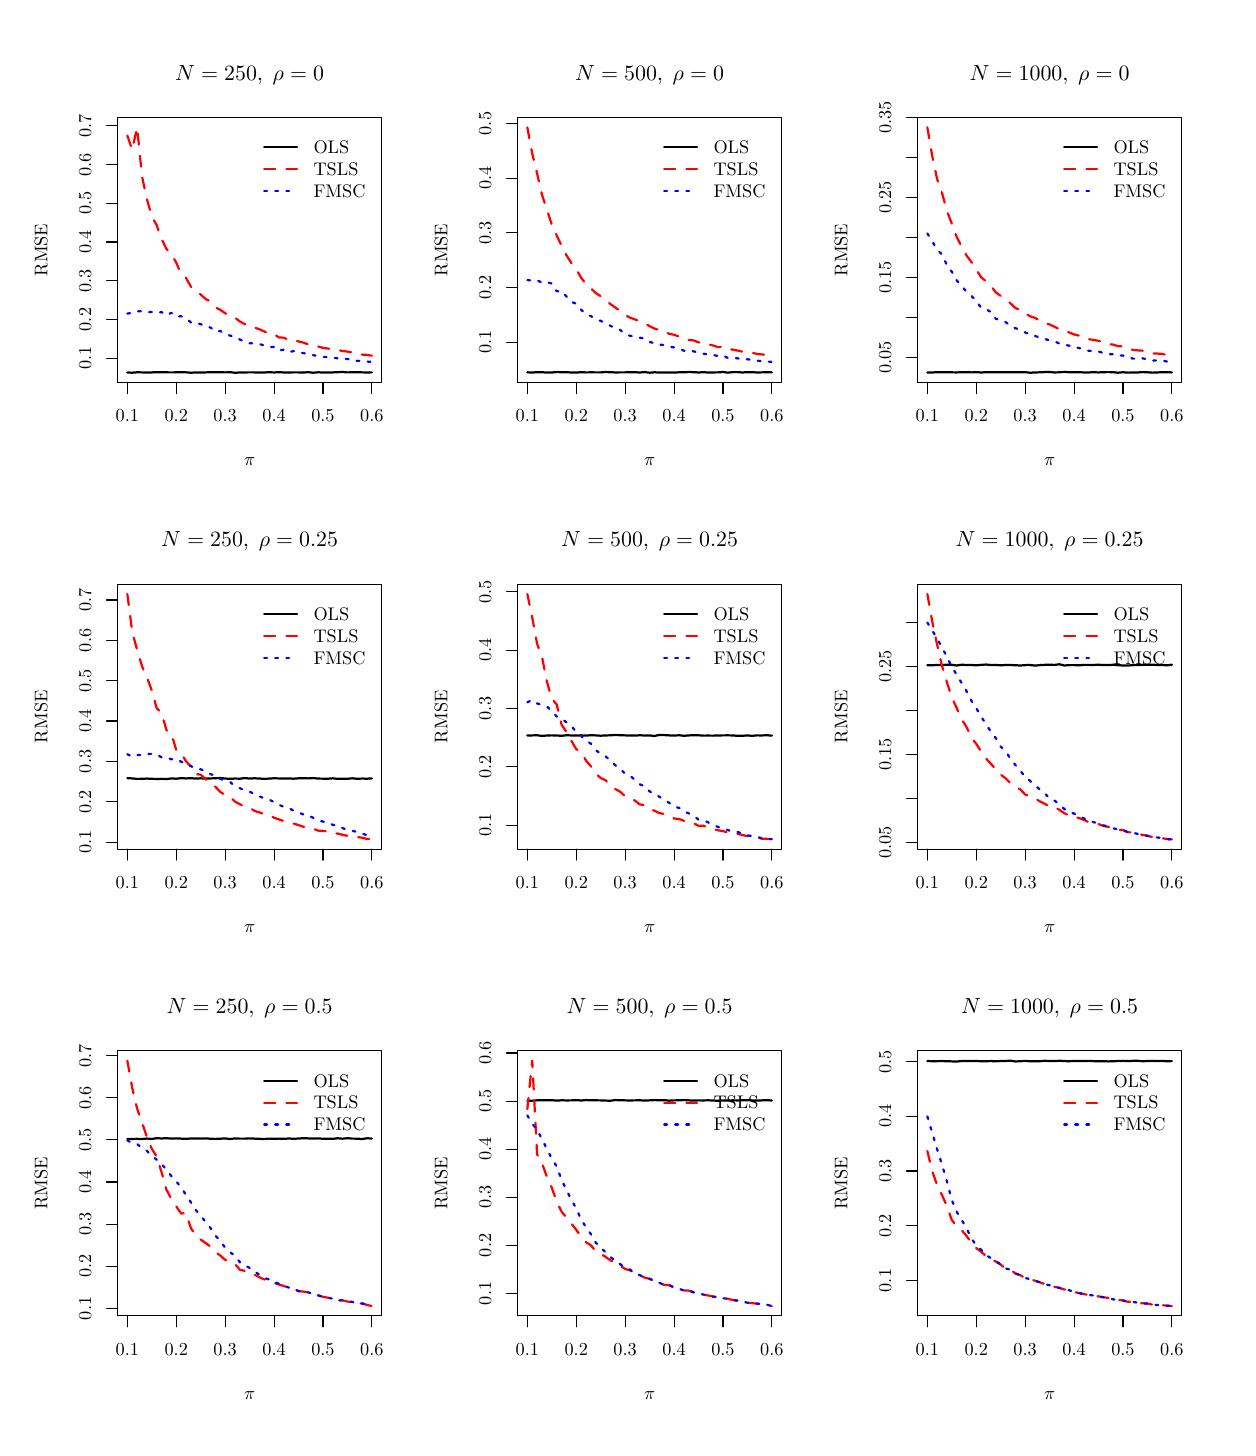
\begin{tikzpicture}[x=1pt,y=1pt]
\definecolor[named]{fillColor}{rgb}{1.00,1.00,1.00}
\path[use as bounding box,fill=fillColor,fill opacity=0.00] (0,0) rectangle (433.62,505.89);
\begin{scope}
\path[clip] ( 32.47,377.65) rectangle (127.91,473.42);
\definecolor[named]{drawColor}{rgb}{0.00,0.00,0.00}

\path[draw=drawColor,line width= 0.8pt,line join=round,line cap=round] ( 36.01,381.28) --
	( 37.77,381.21) --
	( 39.54,381.36) --
	( 41.31,381.32) --
	( 43.08,381.27) --
	( 44.84,381.31) --
	( 46.61,381.41) --
	( 48.38,381.34) --
	( 50.15,381.34) --
	( 51.91,381.32) --
	( 53.68,381.34) --
	( 55.45,381.35) --
	( 57.21,381.34) --
	( 58.98,381.20) --
	( 60.75,381.31) --
	( 62.52,381.29) --
	( 64.28,381.32) --
	( 66.05,381.38) --
	( 67.82,381.35) --
	( 69.59,381.41) --
	( 71.35,381.32) --
	( 73.12,381.40) --
	( 74.89,381.20) --
	( 76.66,381.27) --
	( 78.42,381.31) --
	( 80.19,381.33) --
	( 81.96,381.32) --
	( 83.72,381.27) --
	( 85.49,381.30) --
	( 87.26,381.38) --
	( 89.03,381.30) --
	( 90.79,381.39) --
	( 92.56,381.30) --
	( 94.33,381.29) --
	( 96.10,381.33) --
	( 97.86,381.32) --
	( 99.63,381.28) --
	(101.40,381.38) --
	(103.17,381.20) --
	(104.93,381.35) --
	(106.70,381.29) --
	(108.47,381.25) --
	(110.23,381.32) --
	(112.00,381.40) --
	(113.77,381.47) --
	(115.54,381.33) --
	(117.30,381.34) --
	(119.07,381.38) --
	(120.84,381.33) --
	(122.61,381.30) --
	(124.37,381.33);
\end{scope}
\begin{scope}
\path[clip] (  0.00,  0.00) rectangle (433.62,505.89);
\definecolor[named]{drawColor}{rgb}{0.00,0.00,0.00}

\path[draw=drawColor,line width= 0.4pt,line join=round,line cap=round] ( 36.01,377.65) -- (124.37,377.65);

\path[draw=drawColor,line width= 0.4pt,line join=round,line cap=round] ( 36.01,377.65) -- ( 36.01,373.69);

\path[draw=drawColor,line width= 0.4pt,line join=round,line cap=round] ( 53.68,377.65) -- ( 53.68,373.69);

\path[draw=drawColor,line width= 0.4pt,line join=round,line cap=round] ( 71.35,377.65) -- ( 71.35,373.69);

\path[draw=drawColor,line width= 0.4pt,line join=round,line cap=round] ( 89.03,377.65) -- ( 89.03,373.69);

\path[draw=drawColor,line width= 0.4pt,line join=round,line cap=round] (106.70,377.65) -- (106.70,373.69);

\path[draw=drawColor,line width= 0.4pt,line join=round,line cap=round] (124.37,377.65) -- (124.37,373.69);

\node[text=drawColor,anchor=base,inner sep=0pt, outer sep=0pt, scale=  0.66] at ( 36.01,363.40) {0.1};

\node[text=drawColor,anchor=base,inner sep=0pt, outer sep=0pt, scale=  0.66] at ( 53.68,363.40) {0.2};

\node[text=drawColor,anchor=base,inner sep=0pt, outer sep=0pt, scale=  0.66] at ( 71.35,363.40) {0.3};

\node[text=drawColor,anchor=base,inner sep=0pt, outer sep=0pt, scale=  0.66] at ( 89.03,363.40) {0.4};

\node[text=drawColor,anchor=base,inner sep=0pt, outer sep=0pt, scale=  0.66] at (106.70,363.40) {0.5};

\node[text=drawColor,anchor=base,inner sep=0pt, outer sep=0pt, scale=  0.66] at (124.37,363.40) {0.6};

\path[draw=drawColor,line width= 0.4pt,line join=round,line cap=round] ( 32.47,386.43) -- ( 32.47,470.42);

\path[draw=drawColor,line width= 0.4pt,line join=round,line cap=round] ( 32.47,386.43) -- ( 28.51,386.43);

\path[draw=drawColor,line width= 0.4pt,line join=round,line cap=round] ( 32.47,400.43) -- ( 28.51,400.43);

\path[draw=drawColor,line width= 0.4pt,line join=round,line cap=round] ( 32.47,414.43) -- ( 28.51,414.43);

\path[draw=drawColor,line width= 0.4pt,line join=round,line cap=round] ( 32.47,428.43) -- ( 28.51,428.43);

\path[draw=drawColor,line width= 0.4pt,line join=round,line cap=round] ( 32.47,442.43) -- ( 28.51,442.43);

\path[draw=drawColor,line width= 0.4pt,line join=round,line cap=round] ( 32.47,456.42) -- ( 28.51,456.42);

\path[draw=drawColor,line width= 0.4pt,line join=round,line cap=round] ( 32.47,470.42) -- ( 28.51,470.42);

\node[text=drawColor,rotate= 90.00,anchor=base,inner sep=0pt, outer sep=0pt, scale=  0.66] at ( 22.97,386.43) {0.1};

\node[text=drawColor,rotate= 90.00,anchor=base,inner sep=0pt, outer sep=0pt, scale=  0.66] at ( 22.97,400.43) {0.2};

\node[text=drawColor,rotate= 90.00,anchor=base,inner sep=0pt, outer sep=0pt, scale=  0.66] at ( 22.97,414.43) {0.3};

\node[text=drawColor,rotate= 90.00,anchor=base,inner sep=0pt, outer sep=0pt, scale=  0.66] at ( 22.97,428.43) {0.4};

\node[text=drawColor,rotate= 90.00,anchor=base,inner sep=0pt, outer sep=0pt, scale=  0.66] at ( 22.97,442.43) {0.5};

\node[text=drawColor,rotate= 90.00,anchor=base,inner sep=0pt, outer sep=0pt, scale=  0.66] at ( 22.97,456.42) {0.6};

\node[text=drawColor,rotate= 90.00,anchor=base,inner sep=0pt, outer sep=0pt, scale=  0.66] at ( 22.97,470.42) {0.7};

\path[draw=drawColor,line width= 0.4pt,line join=round,line cap=round] ( 32.47,377.65) --
	(127.91,377.65) --
	(127.91,473.42) --
	( 32.47,473.42) --
	( 32.47,377.65);
\end{scope}
\begin{scope}
\path[clip] (  0.00,337.26) rectangle (144.54,505.89);
\definecolor[named]{drawColor}{rgb}{0.00,0.00,0.00}

\node[text=drawColor,anchor=base,inner sep=0pt, outer sep=0pt, scale=  0.79] at ( 80.19,486.92) {\bfseries $N=250, \;\rho=0$};

\node[text=drawColor,anchor=base,inner sep=0pt, outer sep=0pt, scale=  0.66] at ( 80.19,347.56) {$\pi$};

\node[text=drawColor,rotate= 90.00,anchor=base,inner sep=0pt, outer sep=0pt, scale=  0.66] at (  7.13,425.53) {RMSE};
\end{scope}
\begin{scope}
\path[clip] ( 32.47,377.65) rectangle (127.91,473.42);
\definecolor[named]{drawColor}{rgb}{1.00,0.00,0.00}

\path[draw=drawColor,line width= 0.8pt,dash pattern=on 4pt off 4pt ,line join=round,line cap=round] ( 36.01,466.90) --
	( 37.77,461.77) --
	( 39.54,469.87) --
	( 41.31,452.21) --
	( 43.08,443.93) --
	( 44.84,437.71) --
	( 46.61,434.52) --
	( 48.38,429.50) --
	( 50.15,425.93) --
	( 51.91,424.10) --
	( 53.68,420.96) --
	( 55.45,416.99) --
	( 57.21,415.46) --
	( 58.98,412.33) --
	( 60.75,410.79) --
	( 62.52,409.47) --
	( 64.28,407.85) --
	( 66.05,406.94) --
	( 67.82,404.82) --
	( 69.59,403.93) --
	( 71.35,402.71) --
	( 73.12,401.68) --
	( 74.89,401.08) --
	( 76.66,399.74) --
	( 78.42,398.79) --
	( 80.19,397.80) --
	( 81.96,397.51) --
	( 83.72,396.91) --
	( 85.49,396.12) --
	( 87.26,395.31) --
	( 89.03,395.19) --
	( 90.79,393.94) --
	( 92.56,393.87) --
	( 94.33,393.00) --
	( 96.10,393.04) --
	( 97.86,392.50) --
	( 99.63,392.08) --
	(101.40,391.47) --
	(103.17,391.07) --
	(104.93,390.70) --
	(106.70,390.17) --
	(108.47,389.94) --
	(110.23,389.63) --
	(112.00,389.41) --
	(113.77,389.06) --
	(115.54,388.83) --
	(117.30,388.55) --
	(119.07,388.06) --
	(120.84,387.77) --
	(122.61,387.62) --
	(124.37,387.36);
\definecolor[named]{drawColor}{rgb}{0.00,0.00,1.00}

\path[draw=drawColor,line width= 0.8pt,dash pattern=on 1pt off 3pt ,line join=round,line cap=round] ( 36.01,402.56) --
	( 37.77,402.87) --
	( 39.54,403.36) --
	( 41.31,403.47) --
	( 43.08,403.12) --
	( 44.84,403.14) --
	( 46.61,402.82) --
	( 48.38,403.13) --
	( 50.15,401.89) --
	( 51.91,402.85) --
	( 53.68,401.46) --
	( 55.45,401.61) --
	( 57.21,400.92) --
	( 58.98,399.37) --
	( 60.75,399.19) --
	( 62.52,398.76) --
	( 64.28,397.82) --
	( 66.05,397.55) --
	( 67.82,396.06) --
	( 69.59,396.28) --
	( 71.35,395.10) --
	( 73.12,394.62) --
	( 74.89,394.18) --
	( 76.66,393.20) --
	( 78.42,392.47) --
	( 80.19,391.83) --
	( 81.96,391.79) --
	( 83.72,391.56) --
	( 85.49,391.06) --
	( 87.26,390.48) --
	( 89.03,390.54) --
	( 90.79,389.21) --
	( 92.56,389.54) --
	( 94.33,388.62) --
	( 96.10,389.01) --
	( 97.86,388.57) --
	( 99.63,388.29) --
	(101.40,387.97) --
	(103.17,387.55) --
	(104.93,387.18) --
	(106.70,386.95) --
	(108.47,386.80) --
	(110.23,386.52) --
	(112.00,386.45) --
	(113.77,386.35) --
	(115.54,386.13) --
	(117.30,386.00) --
	(119.07,385.50) --
	(120.84,385.44) --
	(122.61,385.24) --
	(124.37,385.10);
\definecolor[named]{drawColor}{rgb}{0.00,0.00,0.00}

\path[draw=drawColor,line width= 0.8pt,line join=round,line cap=round] ( 85.47,462.63) -- ( 97.35,462.63);
\definecolor[named]{drawColor}{rgb}{1.00,0.00,0.00}

\path[draw=drawColor,line width= 0.8pt,dash pattern=on 4pt off 4pt ,line join=round,line cap=round] ( 85.47,454.71) -- ( 97.35,454.71);
\definecolor[named]{drawColor}{rgb}{0.00,0.00,1.00}

\path[draw=drawColor,line width= 0.8pt,dash pattern=on 1pt off 3pt ,line join=round,line cap=round] ( 85.47,446.79) -- ( 97.35,446.79);
\definecolor[named]{drawColor}{rgb}{0.00,0.00,0.00}

\node[text=drawColor,anchor=base west,inner sep=0pt, outer sep=0pt, scale=  0.66] at (103.29,460.35) {OLS};

\node[text=drawColor,anchor=base west,inner sep=0pt, outer sep=0pt, scale=  0.66] at (103.29,452.43) {TSLS};

\node[text=drawColor,anchor=base west,inner sep=0pt, outer sep=0pt, scale=  0.66] at (103.29,444.51) {FMSC};
\end{scope}
\begin{scope}
\path[clip] (177.01,377.65) rectangle (272.45,473.42);
\definecolor[named]{drawColor}{rgb}{0.00,0.00,0.00}

\path[draw=drawColor,line width= 0.8pt,line join=round,line cap=round] (180.55,381.35) --
	(182.31,381.27) --
	(184.08,381.41) --
	(185.85,381.36) --
	(187.62,381.28) --
	(189.38,381.28) --
	(191.15,381.46) --
	(192.92,381.37) --
	(194.69,381.36) --
	(196.45,381.30) --
	(198.22,381.25) --
	(199.99,381.38) --
	(201.75,381.32) --
	(203.52,381.34) --
	(205.29,381.33) --
	(207.06,381.32) --
	(208.82,381.45) --
	(210.59,381.38) --
	(212.36,381.30) --
	(214.13,381.33) --
	(215.89,381.33) --
	(217.66,381.39) --
	(219.43,381.38) --
	(221.20,381.28) --
	(222.96,381.44) --
	(224.73,381.20) --
	(226.50,381.36) --
	(228.26,381.27) --
	(230.03,381.32) --
	(231.80,381.28) --
	(233.57,381.26) --
	(235.33,381.35) --
	(237.10,381.36) --
	(238.87,381.44) --
	(240.64,381.40) --
	(242.40,381.29) --
	(244.17,381.39) --
	(245.94,381.28) --
	(247.71,381.31) --
	(249.47,381.33) --
	(251.24,381.47) --
	(253.01,381.22) --
	(254.77,381.41) --
	(256.54,381.42) --
	(258.31,381.29) --
	(260.08,381.40) --
	(261.84,381.39) --
	(263.61,381.29) --
	(265.38,381.33) --
	(267.15,381.38) --
	(268.91,381.35);
\end{scope}
\begin{scope}
\path[clip] (  0.00,  0.00) rectangle (433.62,505.89);
\definecolor[named]{drawColor}{rgb}{0.00,0.00,0.00}

\path[draw=drawColor,line width= 0.4pt,line join=round,line cap=round] (180.55,377.65) -- (268.91,377.65);

\path[draw=drawColor,line width= 0.4pt,line join=round,line cap=round] (180.55,377.65) -- (180.55,373.69);

\path[draw=drawColor,line width= 0.4pt,line join=round,line cap=round] (198.22,377.65) -- (198.22,373.69);

\path[draw=drawColor,line width= 0.4pt,line join=round,line cap=round] (215.89,377.65) -- (215.89,373.69);

\path[draw=drawColor,line width= 0.4pt,line join=round,line cap=round] (233.57,377.65) -- (233.57,373.69);

\path[draw=drawColor,line width= 0.4pt,line join=round,line cap=round] (251.24,377.65) -- (251.24,373.69);

\path[draw=drawColor,line width= 0.4pt,line join=round,line cap=round] (268.91,377.65) -- (268.91,373.69);

\node[text=drawColor,anchor=base,inner sep=0pt, outer sep=0pt, scale=  0.66] at (180.55,363.40) {0.1};

\node[text=drawColor,anchor=base,inner sep=0pt, outer sep=0pt, scale=  0.66] at (198.22,363.40) {0.2};

\node[text=drawColor,anchor=base,inner sep=0pt, outer sep=0pt, scale=  0.66] at (215.89,363.40) {0.3};

\node[text=drawColor,anchor=base,inner sep=0pt, outer sep=0pt, scale=  0.66] at (233.57,363.40) {0.4};

\node[text=drawColor,anchor=base,inner sep=0pt, outer sep=0pt, scale=  0.66] at (251.24,363.40) {0.5};

\node[text=drawColor,anchor=base,inner sep=0pt, outer sep=0pt, scale=  0.66] at (268.91,363.40) {0.6};

\path[draw=drawColor,line width= 0.4pt,line join=round,line cap=round] (177.01,392.25) -- (177.01,471.27);

\path[draw=drawColor,line width= 0.4pt,line join=round,line cap=round] (177.01,392.25) -- (173.05,392.25);

\path[draw=drawColor,line width= 0.4pt,line join=round,line cap=round] (177.01,412.01) -- (173.05,412.01);

\path[draw=drawColor,line width= 0.4pt,line join=round,line cap=round] (177.01,431.76) -- (173.05,431.76);

\path[draw=drawColor,line width= 0.4pt,line join=round,line cap=round] (177.01,451.52) -- (173.05,451.52);

\path[draw=drawColor,line width= 0.4pt,line join=round,line cap=round] (177.01,471.27) -- (173.05,471.27);

\node[text=drawColor,rotate= 90.00,anchor=base,inner sep=0pt, outer sep=0pt, scale=  0.66] at (167.51,392.25) {0.1};

\node[text=drawColor,rotate= 90.00,anchor=base,inner sep=0pt, outer sep=0pt, scale=  0.66] at (167.51,412.01) {0.2};

\node[text=drawColor,rotate= 90.00,anchor=base,inner sep=0pt, outer sep=0pt, scale=  0.66] at (167.51,431.76) {0.3};

\node[text=drawColor,rotate= 90.00,anchor=base,inner sep=0pt, outer sep=0pt, scale=  0.66] at (167.51,451.52) {0.4};

\node[text=drawColor,rotate= 90.00,anchor=base,inner sep=0pt, outer sep=0pt, scale=  0.66] at (167.51,471.27) {0.5};

\path[draw=drawColor,line width= 0.4pt,line join=round,line cap=round] (177.01,377.65) --
	(272.45,377.65) --
	(272.45,473.42) --
	(177.01,473.42) --
	(177.01,377.65);
\end{scope}
\begin{scope}
\path[clip] (144.54,337.26) rectangle (289.08,505.89);
\definecolor[named]{drawColor}{rgb}{0.00,0.00,0.00}

\node[text=drawColor,anchor=base,inner sep=0pt, outer sep=0pt, scale=  0.79] at (224.73,486.92) {\bfseries $N=500, \;\rho=0$};

\node[text=drawColor,anchor=base,inner sep=0pt, outer sep=0pt, scale=  0.66] at (224.73,347.56) {$\pi$};

\node[text=drawColor,rotate= 90.00,anchor=base,inner sep=0pt, outer sep=0pt, scale=  0.66] at (151.67,425.53) {RMSE};
\end{scope}
\begin{scope}
\path[clip] (177.01,377.65) rectangle (272.45,473.42);
\definecolor[named]{drawColor}{rgb}{1.00,0.00,0.00}

\path[draw=drawColor,line width= 0.8pt,dash pattern=on 4pt off 4pt ,line join=round,line cap=round] (180.55,469.87) --
	(182.31,460.41) --
	(184.08,453.21) --
	(185.85,445.46) --
	(187.62,440.10) --
	(189.38,434.78) --
	(191.15,430.82) --
	(192.92,427.12) --
	(194.69,423.65) --
	(196.45,420.82) --
	(198.22,418.57) --
	(199.99,415.52) --
	(201.75,413.23) --
	(203.52,411.66) --
	(205.29,409.99) --
	(207.06,408.86) --
	(208.82,407.34) --
	(210.59,405.99) --
	(212.36,404.74) --
	(214.13,403.52) --
	(215.89,402.02) --
	(217.66,401.10) --
	(219.43,400.45) --
	(221.20,399.82) --
	(222.96,399.09) --
	(224.73,398.02) --
	(226.50,397.16) --
	(228.26,396.61) --
	(230.03,395.99) --
	(231.80,395.28) --
	(233.57,394.92) --
	(235.33,394.28) --
	(237.10,393.38) --
	(238.87,393.02) --
	(240.64,392.87) --
	(242.40,392.18) --
	(244.17,391.74) --
	(245.94,391.47) --
	(247.71,391.03) --
	(249.47,390.46) --
	(251.24,390.62) --
	(253.01,389.73) --
	(254.77,389.56) --
	(256.54,389.21) --
	(258.31,388.80) --
	(260.08,388.69) --
	(261.84,388.38) --
	(263.61,387.99) --
	(265.38,387.81) --
	(267.15,387.58) --
	(268.91,387.30);
\definecolor[named]{drawColor}{rgb}{0.00,0.00,1.00}

\path[draw=drawColor,line width= 0.8pt,dash pattern=on 1pt off 3pt ,line join=round,line cap=round] (180.55,414.68) --
	(182.31,414.53) --
	(184.08,414.62) --
	(185.85,413.72) --
	(187.62,413.92) --
	(189.38,413.42) --
	(191.15,410.65) --
	(192.92,410.73) --
	(194.69,408.76) --
	(196.45,406.83) --
	(198.22,406.11) --
	(199.99,403.96) --
	(201.75,402.36) --
	(203.52,401.66) --
	(205.29,400.62) --
	(207.06,399.93) --
	(208.82,399.12) --
	(210.59,398.13) --
	(212.36,397.28) --
	(214.13,396.65) --
	(215.89,395.09) --
	(217.66,394.54) --
	(219.43,394.23) --
	(221.20,393.85) --
	(222.96,393.49) --
	(224.73,392.33) --
	(226.50,391.84) --
	(228.26,391.36) --
	(230.03,391.19) --
	(231.80,390.58) --
	(233.57,390.34) --
	(235.33,389.94) --
	(237.10,389.16) --
	(238.87,388.91) --
	(240.64,388.94) --
	(242.40,388.37) --
	(244.17,388.05) --
	(245.94,387.86) --
	(247.71,387.63) --
	(249.47,387.22) --
	(251.24,387.39) --
	(253.01,386.54) --
	(254.77,386.69) --
	(256.54,386.39) --
	(258.31,385.99) --
	(260.08,386.07) --
	(261.84,385.77) --
	(263.61,385.53) --
	(265.38,385.40) --
	(267.15,385.29) --
	(268.91,385.10);
\definecolor[named]{drawColor}{rgb}{0.00,0.00,0.00}

\path[draw=drawColor,line width= 0.8pt,line join=round,line cap=round] (230.01,462.63) -- (241.89,462.63);
\definecolor[named]{drawColor}{rgb}{1.00,0.00,0.00}

\path[draw=drawColor,line width= 0.8pt,dash pattern=on 4pt off 4pt ,line join=round,line cap=round] (230.01,454.71) -- (241.89,454.71);
\definecolor[named]{drawColor}{rgb}{0.00,0.00,1.00}

\path[draw=drawColor,line width= 0.8pt,dash pattern=on 1pt off 3pt ,line join=round,line cap=round] (230.01,446.79) -- (241.89,446.79);
\definecolor[named]{drawColor}{rgb}{0.00,0.00,0.00}

\node[text=drawColor,anchor=base west,inner sep=0pt, outer sep=0pt, scale=  0.66] at (247.83,460.35) {OLS};

\node[text=drawColor,anchor=base west,inner sep=0pt, outer sep=0pt, scale=  0.66] at (247.83,452.43) {TSLS};

\node[text=drawColor,anchor=base west,inner sep=0pt, outer sep=0pt, scale=  0.66] at (247.83,444.51) {FMSC};
\end{scope}
\begin{scope}
\path[clip] (321.55,377.65) rectangle (416.99,473.42);
\definecolor[named]{drawColor}{rgb}{0.00,0.00,0.00}

\path[draw=drawColor,line width= 0.8pt,line join=round,line cap=round] (325.09,381.27) --
	(326.85,381.29) --
	(328.62,381.40) --
	(330.39,381.35) --
	(332.16,381.36) --
	(333.92,381.34) --
	(335.69,381.31) --
	(337.46,381.41) --
	(339.23,381.41) --
	(340.99,381.32) --
	(342.76,381.41) --
	(344.53,381.29) --
	(346.29,381.38) --
	(348.06,381.39) --
	(349.83,381.40) --
	(351.60,381.36) --
	(353.36,381.34) --
	(355.13,381.35) --
	(356.90,381.38) --
	(358.67,381.39) --
	(360.43,381.41) --
	(362.20,381.20) --
	(363.97,381.30) --
	(365.74,381.34) --
	(367.50,381.44) --
	(369.27,381.48) --
	(371.04,381.30) --
	(372.80,381.35) --
	(374.57,381.52) --
	(376.34,381.36) --
	(378.11,381.36) --
	(379.87,381.39) --
	(381.64,381.31) --
	(383.41,381.31) --
	(385.18,381.37) --
	(386.94,381.31) --
	(388.71,381.40) --
	(390.48,381.42) --
	(392.25,381.38) --
	(394.01,381.21) --
	(395.78,381.37) --
	(397.55,381.23) --
	(399.31,381.28) --
	(401.08,381.29) --
	(402.85,381.43) --
	(404.62,381.36) --
	(406.38,381.23) --
	(408.15,381.30) --
	(409.92,381.38) --
	(411.69,381.40) --
	(413.45,381.31);
\end{scope}
\begin{scope}
\path[clip] (  0.00,  0.00) rectangle (433.62,505.89);
\definecolor[named]{drawColor}{rgb}{0.00,0.00,0.00}

\path[draw=drawColor,line width= 0.4pt,line join=round,line cap=round] (325.09,377.65) -- (413.45,377.65);

\path[draw=drawColor,line width= 0.4pt,line join=round,line cap=round] (325.09,377.65) -- (325.09,373.69);

\path[draw=drawColor,line width= 0.4pt,line join=round,line cap=round] (342.76,377.65) -- (342.76,373.69);

\path[draw=drawColor,line width= 0.4pt,line join=round,line cap=round] (360.43,377.65) -- (360.43,373.69);

\path[draw=drawColor,line width= 0.4pt,line join=round,line cap=round] (378.11,377.65) -- (378.11,373.69);

\path[draw=drawColor,line width= 0.4pt,line join=round,line cap=round] (395.78,377.65) -- (395.78,373.69);

\path[draw=drawColor,line width= 0.4pt,line join=round,line cap=round] (413.45,377.65) -- (413.45,373.69);

\node[text=drawColor,anchor=base,inner sep=0pt, outer sep=0pt, scale=  0.66] at (325.09,363.40) {0.1};

\node[text=drawColor,anchor=base,inner sep=0pt, outer sep=0pt, scale=  0.66] at (342.76,363.40) {0.2};

\node[text=drawColor,anchor=base,inner sep=0pt, outer sep=0pt, scale=  0.66] at (360.43,363.40) {0.3};

\node[text=drawColor,anchor=base,inner sep=0pt, outer sep=0pt, scale=  0.66] at (378.11,363.40) {0.4};

\node[text=drawColor,anchor=base,inner sep=0pt, outer sep=0pt, scale=  0.66] at (395.78,363.40) {0.5};

\node[text=drawColor,anchor=base,inner sep=0pt, outer sep=0pt, scale=  0.66] at (413.45,363.40) {0.6};

\path[draw=drawColor,line width= 0.4pt,line join=round,line cap=round] (321.55,386.65) -- (321.55,473.35);

\path[draw=drawColor,line width= 0.4pt,line join=round,line cap=round] (321.55,386.65) -- (317.59,386.65);

\path[draw=drawColor,line width= 0.4pt,line join=round,line cap=round] (321.55,401.10) -- (317.59,401.10);

\path[draw=drawColor,line width= 0.4pt,line join=round,line cap=round] (321.55,415.55) -- (317.59,415.55);

\path[draw=drawColor,line width= 0.4pt,line join=round,line cap=round] (321.55,430.00) -- (317.59,430.00);

\path[draw=drawColor,line width= 0.4pt,line join=round,line cap=round] (321.55,444.45) -- (317.59,444.45);

\path[draw=drawColor,line width= 0.4pt,line join=round,line cap=round] (321.55,458.90) -- (317.59,458.90);

\path[draw=drawColor,line width= 0.4pt,line join=round,line cap=round] (321.55,473.35) -- (317.59,473.35);

\node[text=drawColor,rotate= 90.00,anchor=base,inner sep=0pt, outer sep=0pt, scale=  0.66] at (312.05,386.65) {0.05};

\node[text=drawColor,rotate= 90.00,anchor=base,inner sep=0pt, outer sep=0pt, scale=  0.66] at (312.05,415.55) {0.15};

\node[text=drawColor,rotate= 90.00,anchor=base,inner sep=0pt, outer sep=0pt, scale=  0.66] at (312.05,444.45) {0.25};

\node[text=drawColor,rotate= 90.00,anchor=base,inner sep=0pt, outer sep=0pt, scale=  0.66] at (312.05,473.35) {0.35};

\path[draw=drawColor,line width= 0.4pt,line join=round,line cap=round] (321.55,377.65) --
	(416.99,377.65) --
	(416.99,473.42) --
	(321.55,473.42) --
	(321.55,377.65);
\end{scope}
\begin{scope}
\path[clip] (289.08,337.26) rectangle (433.62,505.89);
\definecolor[named]{drawColor}{rgb}{0.00,0.00,0.00}

\node[text=drawColor,anchor=base,inner sep=0pt, outer sep=0pt, scale=  0.79] at (369.27,486.92) {\bfseries $N=1000, \;\rho=0$};

\node[text=drawColor,anchor=base,inner sep=0pt, outer sep=0pt, scale=  0.66] at (369.27,347.56) {$\pi$};

\node[text=drawColor,rotate= 90.00,anchor=base,inner sep=0pt, outer sep=0pt, scale=  0.66] at (296.21,425.53) {RMSE};
\end{scope}
\begin{scope}
\path[clip] (321.55,377.65) rectangle (416.99,473.42);
\definecolor[named]{drawColor}{rgb}{1.00,0.00,0.00}

\path[draw=drawColor,line width= 0.8pt,dash pattern=on 4pt off 4pt ,line join=round,line cap=round] (325.09,469.87) --
	(326.85,459.55) --
	(328.62,451.20) --
	(330.39,446.20) --
	(332.16,439.70) --
	(333.92,435.07) --
	(335.69,430.30) --
	(337.46,426.80) --
	(339.23,423.59) --
	(340.99,421.24) --
	(342.76,418.49) --
	(344.53,415.67) --
	(346.29,414.26) --
	(348.06,412.60) --
	(349.83,410.21) --
	(351.60,408.99) --
	(353.36,407.81) --
	(355.13,406.28) --
	(356.90,404.59) --
	(358.67,403.90) --
	(360.43,402.60) --
	(362.20,401.63) --
	(363.97,401.04) --
	(365.74,400.01) --
	(367.50,399.22) --
	(369.27,398.62) --
	(371.04,397.80) --
	(372.80,396.92) --
	(374.57,396.26) --
	(376.34,395.75) --
	(378.11,395.05) --
	(379.87,394.60) --
	(381.64,393.84) --
	(383.41,393.32) --
	(385.18,393.04) --
	(386.94,392.74) --
	(388.71,392.11) --
	(390.48,391.59) --
	(392.25,391.35) --
	(394.01,390.80) --
	(395.78,390.67) --
	(397.55,390.24) --
	(399.31,389.45) --
	(401.08,389.28) --
	(402.85,389.17) --
	(404.62,388.81) --
	(406.38,388.21) --
	(408.15,388.12) --
	(409.92,387.99) --
	(411.69,387.57) --
	(413.45,387.36);
\definecolor[named]{drawColor}{rgb}{0.00,0.00,1.00}

\path[draw=drawColor,line width= 0.8pt,dash pattern=on 1pt off 3pt ,line join=round,line cap=round] (325.09,431.52) --
	(326.85,428.76) --
	(328.62,425.55) --
	(330.39,423.97) --
	(332.16,420.11) --
	(333.92,417.72) --
	(335.69,414.57) --
	(337.46,412.58) --
	(339.23,410.45) --
	(340.99,408.96) --
	(342.76,407.18) --
	(344.53,404.61) --
	(346.29,404.17) --
	(348.06,403.13) --
	(349.83,400.69) --
	(351.60,400.18) --
	(353.36,399.48) --
	(355.13,398.16) --
	(356.90,397.27) --
	(358.67,396.79) --
	(360.43,395.77) --
	(362.20,395.05) --
	(363.97,394.50) --
	(365.74,393.93) --
	(367.50,393.42) --
	(369.27,392.86) --
	(371.04,392.54) --
	(372.80,391.74) --
	(374.57,391.36) --
	(376.34,390.96) --
	(378.11,390.35) --
	(379.87,390.16) --
	(381.64,389.41) --
	(383.41,389.12) --
	(385.18,389.04) --
	(386.94,388.88) --
	(388.71,388.28) --
	(390.48,387.92) --
	(392.25,387.87) --
	(394.01,387.46) --
	(395.78,387.39) --
	(397.55,387.12) --
	(399.31,386.29) --
	(401.08,386.32) --
	(402.85,386.40) --
	(404.62,386.00) --
	(406.38,385.64) --
	(408.15,385.66) --
	(409.92,385.59) --
	(411.69,385.23) --
	(413.45,385.09);
\definecolor[named]{drawColor}{rgb}{0.00,0.00,0.00}

\path[draw=drawColor,line width= 0.8pt,line join=round,line cap=round] (374.55,462.63) -- (386.43,462.63);
\definecolor[named]{drawColor}{rgb}{1.00,0.00,0.00}

\path[draw=drawColor,line width= 0.8pt,dash pattern=on 4pt off 4pt ,line join=round,line cap=round] (374.55,454.71) -- (386.43,454.71);
\definecolor[named]{drawColor}{rgb}{0.00,0.00,1.00}

\path[draw=drawColor,line width= 0.8pt,dash pattern=on 1pt off 3pt ,line join=round,line cap=round] (374.55,446.79) -- (386.43,446.79);
\definecolor[named]{drawColor}{rgb}{0.00,0.00,0.00}

\node[text=drawColor,anchor=base west,inner sep=0pt, outer sep=0pt, scale=  0.66] at (392.37,460.35) {OLS};

\node[text=drawColor,anchor=base west,inner sep=0pt, outer sep=0pt, scale=  0.66] at (392.37,452.43) {TSLS};

\node[text=drawColor,anchor=base west,inner sep=0pt, outer sep=0pt, scale=  0.66] at (392.37,444.51) {FMSC};
\end{scope}
\begin{scope}
\path[clip] ( 32.47,209.02) rectangle (127.91,304.79);
\definecolor[named]{drawColor}{rgb}{0.00,0.00,0.00}

\path[draw=drawColor,line width= 0.8pt,line join=round,line cap=round] ( 36.01,234.72) --
	( 37.77,234.60) --
	( 39.54,234.43) --
	( 41.31,234.46) --
	( 43.08,234.55) --
	( 44.84,234.47) --
	( 46.61,234.40) --
	( 48.38,234.45) --
	( 50.15,234.38) --
	( 51.91,234.59) --
	( 53.68,234.50) --
	( 55.45,234.69) --
	( 57.21,234.60) --
	( 58.98,234.70) --
	( 60.75,234.55) --
	( 62.52,234.64) --
	( 64.28,234.54) --
	( 66.05,234.61) --
	( 67.82,234.65) --
	( 69.59,234.75) --
	( 71.35,234.57) --
	( 73.12,234.45) --
	( 74.89,234.56) --
	( 76.66,234.50) --
	( 78.42,234.73) --
	( 80.19,234.56) --
	( 81.96,234.65) --
	( 83.72,234.57) --
	( 85.49,234.43) --
	( 87.26,234.55) --
	( 89.03,234.65) --
	( 90.79,234.61) --
	( 92.56,234.56) --
	( 94.33,234.58) --
	( 96.10,234.51) --
	( 97.86,234.64) --
	( 99.63,234.66) --
	(101.40,234.62) --
	(103.17,234.73) --
	(104.93,234.55) --
	(106.70,234.52) --
	(108.47,234.49) --
	(110.23,234.64) --
	(112.00,234.44) --
	(113.77,234.51) --
	(115.54,234.46) --
	(117.30,234.65) --
	(119.07,234.47) --
	(120.84,234.55) --
	(122.61,234.50) --
	(124.37,234.62);
\end{scope}
\begin{scope}
\path[clip] (  0.00,  0.00) rectangle (433.62,505.89);
\definecolor[named]{drawColor}{rgb}{0.00,0.00,0.00}

\path[draw=drawColor,line width= 0.4pt,line join=round,line cap=round] ( 36.01,209.02) -- (124.37,209.02);

\path[draw=drawColor,line width= 0.4pt,line join=round,line cap=round] ( 36.01,209.02) -- ( 36.01,205.06);

\path[draw=drawColor,line width= 0.4pt,line join=round,line cap=round] ( 53.68,209.02) -- ( 53.68,205.06);

\path[draw=drawColor,line width= 0.4pt,line join=round,line cap=round] ( 71.35,209.02) -- ( 71.35,205.06);

\path[draw=drawColor,line width= 0.4pt,line join=round,line cap=round] ( 89.03,209.02) -- ( 89.03,205.06);

\path[draw=drawColor,line width= 0.4pt,line join=round,line cap=round] (106.70,209.02) -- (106.70,205.06);

\path[draw=drawColor,line width= 0.4pt,line join=round,line cap=round] (124.37,209.02) -- (124.37,205.06);

\node[text=drawColor,anchor=base,inner sep=0pt, outer sep=0pt, scale=  0.66] at ( 36.01,194.77) {0.1};

\node[text=drawColor,anchor=base,inner sep=0pt, outer sep=0pt, scale=  0.66] at ( 53.68,194.77) {0.2};

\node[text=drawColor,anchor=base,inner sep=0pt, outer sep=0pt, scale=  0.66] at ( 71.35,194.77) {0.3};

\node[text=drawColor,anchor=base,inner sep=0pt, outer sep=0pt, scale=  0.66] at ( 89.03,194.77) {0.4};

\node[text=drawColor,anchor=base,inner sep=0pt, outer sep=0pt, scale=  0.66] at (106.70,194.77) {0.5};

\node[text=drawColor,anchor=base,inner sep=0pt, outer sep=0pt, scale=  0.66] at (124.37,194.77) {0.6};

\path[draw=drawColor,line width= 0.4pt,line join=round,line cap=round] ( 32.47,211.61) -- ( 32.47,299.08);

\path[draw=drawColor,line width= 0.4pt,line join=round,line cap=round] ( 32.47,211.61) -- ( 28.51,211.61);

\path[draw=drawColor,line width= 0.4pt,line join=round,line cap=round] ( 32.47,226.18) -- ( 28.51,226.18);

\path[draw=drawColor,line width= 0.4pt,line join=round,line cap=round] ( 32.47,240.76) -- ( 28.51,240.76);

\path[draw=drawColor,line width= 0.4pt,line join=round,line cap=round] ( 32.47,255.34) -- ( 28.51,255.34);

\path[draw=drawColor,line width= 0.4pt,line join=round,line cap=round] ( 32.47,269.92) -- ( 28.51,269.92);

\path[draw=drawColor,line width= 0.4pt,line join=round,line cap=round] ( 32.47,284.50) -- ( 28.51,284.50);

\path[draw=drawColor,line width= 0.4pt,line join=round,line cap=round] ( 32.47,299.08) -- ( 28.51,299.08);

\node[text=drawColor,rotate= 90.00,anchor=base,inner sep=0pt, outer sep=0pt, scale=  0.66] at ( 22.97,211.61) {0.1};

\node[text=drawColor,rotate= 90.00,anchor=base,inner sep=0pt, outer sep=0pt, scale=  0.66] at ( 22.97,226.18) {0.2};

\node[text=drawColor,rotate= 90.00,anchor=base,inner sep=0pt, outer sep=0pt, scale=  0.66] at ( 22.97,240.76) {0.3};

\node[text=drawColor,rotate= 90.00,anchor=base,inner sep=0pt, outer sep=0pt, scale=  0.66] at ( 22.97,255.34) {0.4};

\node[text=drawColor,rotate= 90.00,anchor=base,inner sep=0pt, outer sep=0pt, scale=  0.66] at ( 22.97,269.92) {0.5};

\node[text=drawColor,rotate= 90.00,anchor=base,inner sep=0pt, outer sep=0pt, scale=  0.66] at ( 22.97,284.50) {0.6};

\node[text=drawColor,rotate= 90.00,anchor=base,inner sep=0pt, outer sep=0pt, scale=  0.66] at ( 22.97,299.08) {0.7};

\path[draw=drawColor,line width= 0.4pt,line join=round,line cap=round] ( 32.47,209.02) --
	(127.91,209.02) --
	(127.91,304.79) --
	( 32.47,304.79) --
	( 32.47,209.02);
\end{scope}
\begin{scope}
\path[clip] (  0.00,168.63) rectangle (144.54,337.26);
\definecolor[named]{drawColor}{rgb}{0.00,0.00,0.00}

\node[text=drawColor,anchor=base,inner sep=0pt, outer sep=0pt, scale=  0.79] at ( 80.19,318.29) {\bfseries $N=250, \;\rho=0.25$};

\node[text=drawColor,anchor=base,inner sep=0pt, outer sep=0pt, scale=  0.66] at ( 80.19,178.93) {$\pi$};

\node[text=drawColor,rotate= 90.00,anchor=base,inner sep=0pt, outer sep=0pt, scale=  0.66] at (  7.13,256.90) {RMSE};
\end{scope}
\begin{scope}
\path[clip] ( 32.47,209.02) rectangle (127.91,304.79);
\definecolor[named]{drawColor}{rgb}{1.00,0.00,0.00}

\path[draw=drawColor,line width= 0.8pt,dash pattern=on 4pt off 4pt ,line join=round,line cap=round] ( 36.01,301.24) --
	( 37.77,287.60) --
	( 39.54,281.05) --
	( 41.31,275.17) --
	( 43.08,271.14) --
	( 44.84,266.48) --
	( 46.61,260.00) --
	( 48.38,258.23) --
	( 50.15,252.04) --
	( 51.91,250.91) --
	( 53.68,244.88) --
	( 55.45,243.78) --
	( 57.21,240.79) --
	( 58.98,238.90) --
	( 60.75,236.17) --
	( 62.52,235.97) --
	( 64.28,234.34) --
	( 66.05,232.79) --
	( 67.82,231.59) --
	( 69.59,229.72) --
	( 71.35,228.60) --
	( 73.12,228.02) --
	( 74.89,226.24) --
	( 76.66,225.27) --
	( 78.42,224.56) --
	( 80.19,224.01) --
	( 81.96,222.88) --
	( 83.72,222.31) --
	( 85.49,221.68) --
	( 87.26,221.42) --
	( 89.03,220.41) --
	( 90.79,219.80) --
	( 92.56,219.17) --
	( 94.33,218.71) --
	( 96.10,218.29) --
	( 97.86,217.73) --
	( 99.63,217.15) --
	(101.40,217.04) --
	(103.17,216.43) --
	(104.93,215.74) --
	(106.70,215.64) --
	(108.47,215.42) --
	(110.23,214.94) --
	(112.00,214.66) --
	(113.77,214.24) --
	(115.54,213.86) --
	(117.30,213.67) --
	(119.07,213.45) --
	(120.84,213.16) --
	(122.61,212.74) --
	(124.37,212.57);
\definecolor[named]{drawColor}{rgb}{0.00,0.00,1.00}

\path[draw=drawColor,line width= 0.8pt,dash pattern=on 1pt off 3pt ,line join=round,line cap=round] ( 36.01,243.37) --
	( 37.77,242.42) --
	( 39.54,243.06) --
	( 41.31,243.09) --
	( 43.08,243.34) --
	( 44.84,243.49) --
	( 46.61,243.15) --
	( 48.38,242.25) --
	( 50.15,242.21) --
	( 51.91,241.53) --
	( 53.68,241.72) --
	( 55.45,240.65) --
	( 57.21,239.57) --
	( 58.98,239.09) --
	( 60.75,237.99) --
	( 62.52,237.89) --
	( 64.28,237.22) --
	( 66.05,236.17) --
	( 67.82,235.55) --
	( 69.59,234.45) --
	( 71.35,233.83) --
	( 73.12,233.35) --
	( 74.89,231.82) --
	( 76.66,231.08) --
	( 78.42,230.27) --
	( 80.19,229.80) --
	( 81.96,228.98) --
	( 83.72,228.14) --
	( 85.49,227.38) --
	( 87.26,226.95) --
	( 89.03,226.07) --
	( 90.79,225.10) --
	( 92.56,224.31) --
	( 94.33,223.87) --
	( 96.10,222.98) --
	( 97.86,222.34) --
	( 99.63,221.57) --
	(101.40,221.34) --
	(103.17,220.35) --
	(104.93,219.38) --
	(106.70,219.02) --
	(108.47,218.51) --
	(110.23,217.88) --
	(112.00,217.30) --
	(113.77,216.66) --
	(115.54,215.98) --
	(117.30,215.70) --
	(119.07,215.21) --
	(120.84,214.63) --
	(122.61,214.13) --
	(124.37,213.72);
\definecolor[named]{drawColor}{rgb}{0.00,0.00,0.00}

\path[draw=drawColor,line width= 0.8pt,line join=round,line cap=round] ( 85.47,294.00) -- ( 97.35,294.00);
\definecolor[named]{drawColor}{rgb}{1.00,0.00,0.00}

\path[draw=drawColor,line width= 0.8pt,dash pattern=on 4pt off 4pt ,line join=round,line cap=round] ( 85.47,286.08) -- ( 97.35,286.08);
\definecolor[named]{drawColor}{rgb}{0.00,0.00,1.00}

\path[draw=drawColor,line width= 0.8pt,dash pattern=on 1pt off 3pt ,line join=round,line cap=round] ( 85.47,278.16) -- ( 97.35,278.16);
\definecolor[named]{drawColor}{rgb}{0.00,0.00,0.00}

\node[text=drawColor,anchor=base west,inner sep=0pt, outer sep=0pt, scale=  0.66] at (103.29,291.72) {OLS};

\node[text=drawColor,anchor=base west,inner sep=0pt, outer sep=0pt, scale=  0.66] at (103.29,283.80) {TSLS};

\node[text=drawColor,anchor=base west,inner sep=0pt, outer sep=0pt, scale=  0.66] at (103.29,275.88) {FMSC};
\end{scope}
\begin{scope}
\path[clip] (177.01,209.02) rectangle (272.45,304.79);
\definecolor[named]{drawColor}{rgb}{0.00,0.00,0.00}

\path[draw=drawColor,line width= 0.8pt,line join=round,line cap=round] (180.55,250.12) --
	(182.31,250.15) --
	(184.08,250.20) --
	(185.85,249.96) --
	(187.62,250.11) --
	(189.38,250.16) --
	(191.15,250.12) --
	(192.92,250.00) --
	(194.69,250.20) --
	(196.45,250.14) --
	(198.22,250.12) --
	(199.99,250.17) --
	(201.75,250.10) --
	(203.52,250.20) --
	(205.29,250.15) --
	(207.06,250.04) --
	(208.82,250.13) --
	(210.59,250.18) --
	(212.36,250.32) --
	(214.13,250.20) --
	(215.89,250.16) --
	(217.66,250.08) --
	(219.43,250.09) --
	(221.20,250.19) --
	(222.96,250.12) --
	(224.73,250.14) --
	(226.50,249.94) --
	(228.26,250.33) --
	(230.03,250.26) --
	(231.80,250.16) --
	(233.57,250.07) --
	(235.33,250.21) --
	(237.10,250.01) --
	(238.87,250.14) --
	(240.64,250.23) --
	(242.40,250.19) --
	(244.17,250.07) --
	(245.94,250.08) --
	(247.71,250.06) --
	(249.47,250.12) --
	(251.24,250.16) --
	(253.01,250.17) --
	(254.77,250.14) --
	(256.54,250.00) --
	(258.31,250.02) --
	(260.08,250.13) --
	(261.84,250.00) --
	(263.61,250.16) --
	(265.38,250.14) --
	(267.15,250.21) --
	(268.91,250.06);
\end{scope}
\begin{scope}
\path[clip] (  0.00,  0.00) rectangle (433.62,505.89);
\definecolor[named]{drawColor}{rgb}{0.00,0.00,0.00}

\path[draw=drawColor,line width= 0.4pt,line join=round,line cap=round] (180.55,209.02) -- (268.91,209.02);

\path[draw=drawColor,line width= 0.4pt,line join=round,line cap=round] (180.55,209.02) -- (180.55,205.06);

\path[draw=drawColor,line width= 0.4pt,line join=round,line cap=round] (198.22,209.02) -- (198.22,205.06);

\path[draw=drawColor,line width= 0.4pt,line join=round,line cap=round] (215.89,209.02) -- (215.89,205.06);

\path[draw=drawColor,line width= 0.4pt,line join=round,line cap=round] (233.57,209.02) -- (233.57,205.06);

\path[draw=drawColor,line width= 0.4pt,line join=round,line cap=round] (251.24,209.02) -- (251.24,205.06);

\path[draw=drawColor,line width= 0.4pt,line join=round,line cap=round] (268.91,209.02) -- (268.91,205.06);

\node[text=drawColor,anchor=base,inner sep=0pt, outer sep=0pt, scale=  0.66] at (180.55,194.77) {0.1};

\node[text=drawColor,anchor=base,inner sep=0pt, outer sep=0pt, scale=  0.66] at (198.22,194.77) {0.2};

\node[text=drawColor,anchor=base,inner sep=0pt, outer sep=0pt, scale=  0.66] at (215.89,194.77) {0.3};

\node[text=drawColor,anchor=base,inner sep=0pt, outer sep=0pt, scale=  0.66] at (233.57,194.77) {0.4};

\node[text=drawColor,anchor=base,inner sep=0pt, outer sep=0pt, scale=  0.66] at (251.24,194.77) {0.5};

\node[text=drawColor,anchor=base,inner sep=0pt, outer sep=0pt, scale=  0.66] at (268.91,194.77) {0.6};

\path[draw=drawColor,line width= 0.4pt,line join=round,line cap=round] (177.01,217.74) -- (177.01,302.02);

\path[draw=drawColor,line width= 0.4pt,line join=round,line cap=round] (177.01,217.74) -- (173.05,217.74);

\path[draw=drawColor,line width= 0.4pt,line join=round,line cap=round] (177.01,238.81) -- (173.05,238.81);

\path[draw=drawColor,line width= 0.4pt,line join=round,line cap=round] (177.01,259.88) -- (173.05,259.88);

\path[draw=drawColor,line width= 0.4pt,line join=round,line cap=round] (177.01,280.95) -- (173.05,280.95);

\path[draw=drawColor,line width= 0.4pt,line join=round,line cap=round] (177.01,302.02) -- (173.05,302.02);

\node[text=drawColor,rotate= 90.00,anchor=base,inner sep=0pt, outer sep=0pt, scale=  0.66] at (167.51,217.74) {0.1};

\node[text=drawColor,rotate= 90.00,anchor=base,inner sep=0pt, outer sep=0pt, scale=  0.66] at (167.51,238.81) {0.2};

\node[text=drawColor,rotate= 90.00,anchor=base,inner sep=0pt, outer sep=0pt, scale=  0.66] at (167.51,259.88) {0.3};

\node[text=drawColor,rotate= 90.00,anchor=base,inner sep=0pt, outer sep=0pt, scale=  0.66] at (167.51,280.95) {0.4};

\node[text=drawColor,rotate= 90.00,anchor=base,inner sep=0pt, outer sep=0pt, scale=  0.66] at (167.51,302.02) {0.5};

\path[draw=drawColor,line width= 0.4pt,line join=round,line cap=round] (177.01,209.02) --
	(272.45,209.02) --
	(272.45,304.79) --
	(177.01,304.79) --
	(177.01,209.02);
\end{scope}
\begin{scope}
\path[clip] (144.54,168.63) rectangle (289.08,337.26);
\definecolor[named]{drawColor}{rgb}{0.00,0.00,0.00}

\node[text=drawColor,anchor=base,inner sep=0pt, outer sep=0pt, scale=  0.79] at (224.73,318.29) {\bfseries $N=500, \;\rho=0.25$};

\node[text=drawColor,anchor=base,inner sep=0pt, outer sep=0pt, scale=  0.66] at (224.73,178.93) {$\pi$};

\node[text=drawColor,rotate= 90.00,anchor=base,inner sep=0pt, outer sep=0pt, scale=  0.66] at (151.67,256.90) {RMSE};
\end{scope}
\begin{scope}
\path[clip] (177.01,209.02) rectangle (272.45,304.79);
\definecolor[named]{drawColor}{rgb}{1.00,0.00,0.00}

\path[draw=drawColor,line width= 0.8pt,dash pattern=on 4pt off 4pt ,line join=round,line cap=round] (180.55,301.24) --
	(182.31,292.78) --
	(184.08,283.24) --
	(185.85,278.53) --
	(187.62,269.57) --
	(189.38,263.35) --
	(191.15,261.36) --
	(192.92,254.05) --
	(194.69,251.35) --
	(196.45,248.21) --
	(198.22,245.19) --
	(199.99,244.13) --
	(201.75,241.04) --
	(203.52,238.98) --
	(205.29,236.31) --
	(207.06,234.76) --
	(208.82,233.94) --
	(210.59,232.24) --
	(212.36,230.74) --
	(214.13,229.77) --
	(215.89,228.12) --
	(217.66,227.60) --
	(219.43,226.56) --
	(221.20,225.19) --
	(222.96,224.98) --
	(224.73,223.48) --
	(226.50,222.93) --
	(228.26,222.09) --
	(230.03,221.72) --
	(231.80,221.03) --
	(233.57,220.13) --
	(235.33,219.93) --
	(237.10,219.32) --
	(238.87,218.83) --
	(240.64,218.44) --
	(242.40,217.45) --
	(244.17,217.49) --
	(245.94,216.90) --
	(247.71,216.34) --
	(249.47,215.84) --
	(251.24,215.56) --
	(253.01,215.07) --
	(254.77,214.56) --
	(256.54,214.59) --
	(258.31,214.15) --
	(260.08,213.76) --
	(261.84,213.51) --
	(263.61,213.31) --
	(265.38,212.80) --
	(267.15,212.77) --
	(268.91,212.57);
\definecolor[named]{drawColor}{rgb}{0.00,0.00,1.00}

\path[draw=drawColor,line width= 0.8pt,dash pattern=on 1pt off 3pt ,line join=round,line cap=round] (180.55,262.12) --
	(182.31,262.92) --
	(184.08,261.70) --
	(185.85,261.11) --
	(187.62,260.62) --
	(189.38,258.83) --
	(191.15,257.00) --
	(192.92,256.23) --
	(194.69,254.86) --
	(196.45,253.56) --
	(198.22,251.36) --
	(199.99,249.94) --
	(201.75,248.35) --
	(203.52,247.15) --
	(205.29,244.82) --
	(207.06,243.51) --
	(208.82,242.60) --
	(210.59,240.91) --
	(212.36,239.37) --
	(214.13,238.06) --
	(215.89,236.31) --
	(217.66,235.59) --
	(219.43,234.05) --
	(221.20,232.49) --
	(222.96,231.74) --
	(224.73,229.94) --
	(226.50,228.96) --
	(228.26,227.97) --
	(230.03,226.77) --
	(231.80,225.80) --
	(233.57,224.36) --
	(235.33,223.97) --
	(237.10,222.77) --
	(238.87,221.95) --
	(240.64,221.14) --
	(242.40,219.72) --
	(244.17,219.58) --
	(245.94,218.67) --
	(247.71,217.90) --
	(249.47,217.04) --
	(251.24,216.54) --
	(253.01,215.97) --
	(254.77,215.26) --
	(256.54,215.24) --
	(258.31,214.67) --
	(260.08,214.08) --
	(261.84,213.73) --
	(263.61,213.52) --
	(265.38,212.94) --
	(267.15,212.84) --
	(268.91,212.65);
\definecolor[named]{drawColor}{rgb}{0.00,0.00,0.00}

\path[draw=drawColor,line width= 0.8pt,line join=round,line cap=round] (230.01,294.00) -- (241.89,294.00);
\definecolor[named]{drawColor}{rgb}{1.00,0.00,0.00}

\path[draw=drawColor,line width= 0.8pt,dash pattern=on 4pt off 4pt ,line join=round,line cap=round] (230.01,286.08) -- (241.89,286.08);
\definecolor[named]{drawColor}{rgb}{0.00,0.00,1.00}

\path[draw=drawColor,line width= 0.8pt,dash pattern=on 1pt off 3pt ,line join=round,line cap=round] (230.01,278.16) -- (241.89,278.16);
\definecolor[named]{drawColor}{rgb}{0.00,0.00,0.00}

\node[text=drawColor,anchor=base west,inner sep=0pt, outer sep=0pt, scale=  0.66] at (247.83,291.72) {OLS};

\node[text=drawColor,anchor=base west,inner sep=0pt, outer sep=0pt, scale=  0.66] at (247.83,283.80) {TSLS};

\node[text=drawColor,anchor=base west,inner sep=0pt, outer sep=0pt, scale=  0.66] at (247.83,275.88) {FMSC};
\end{scope}
\begin{scope}
\path[clip] (321.55,209.02) rectangle (416.99,304.79);
\definecolor[named]{drawColor}{rgb}{0.00,0.00,0.00}

\path[draw=drawColor,line width= 0.8pt,line join=round,line cap=round] (325.09,275.52) --
	(326.85,275.50) --
	(328.62,275.59) --
	(330.39,275.60) --
	(332.16,275.67) --
	(333.92,275.66) --
	(335.69,275.41) --
	(337.46,275.68) --
	(339.23,275.60) --
	(340.99,275.58) --
	(342.76,275.50) --
	(344.53,275.63) --
	(346.29,275.75) --
	(348.06,275.59) --
	(349.83,275.62) --
	(351.60,275.48) --
	(353.36,275.58) --
	(355.13,275.58) --
	(356.90,275.51) --
	(358.67,275.41) --
	(360.43,275.54) --
	(362.20,275.59) --
	(363.97,275.37) --
	(365.74,275.55) --
	(367.50,275.64) --
	(369.27,275.72) --
	(371.04,275.61) --
	(372.80,275.86) --
	(374.57,275.41) --
	(376.34,275.54) --
	(378.11,275.55) --
	(379.87,275.46) --
	(381.64,275.64) --
	(383.41,275.63) --
	(385.18,275.61) --
	(386.94,275.69) --
	(388.71,275.55) --
	(390.48,275.57) --
	(392.25,275.67) --
	(394.01,275.52) --
	(395.78,275.42) --
	(397.55,275.39) --
	(399.31,275.54) --
	(401.08,275.61) --
	(402.85,275.63) --
	(404.62,275.66) --
	(406.38,275.69) --
	(408.15,275.59) --
	(409.92,275.59) --
	(411.69,275.46) --
	(413.45,275.69);
\end{scope}
\begin{scope}
\path[clip] (  0.00,  0.00) rectangle (433.62,505.89);
\definecolor[named]{drawColor}{rgb}{0.00,0.00,0.00}

\path[draw=drawColor,line width= 0.4pt,line join=round,line cap=round] (325.09,209.02) -- (413.45,209.02);

\path[draw=drawColor,line width= 0.4pt,line join=round,line cap=round] (325.09,209.02) -- (325.09,205.06);

\path[draw=drawColor,line width= 0.4pt,line join=round,line cap=round] (342.76,209.02) -- (342.76,205.06);

\path[draw=drawColor,line width= 0.4pt,line join=round,line cap=round] (360.43,209.02) -- (360.43,205.06);

\path[draw=drawColor,line width= 0.4pt,line join=round,line cap=round] (378.11,209.02) -- (378.11,205.06);

\path[draw=drawColor,line width= 0.4pt,line join=round,line cap=round] (395.78,209.02) -- (395.78,205.06);

\path[draw=drawColor,line width= 0.4pt,line join=round,line cap=round] (413.45,209.02) -- (413.45,205.06);

\node[text=drawColor,anchor=base,inner sep=0pt, outer sep=0pt, scale=  0.66] at (325.09,194.77) {0.1};

\node[text=drawColor,anchor=base,inner sep=0pt, outer sep=0pt, scale=  0.66] at (342.76,194.77) {0.2};

\node[text=drawColor,anchor=base,inner sep=0pt, outer sep=0pt, scale=  0.66] at (360.43,194.77) {0.3};

\node[text=drawColor,anchor=base,inner sep=0pt, outer sep=0pt, scale=  0.66] at (378.11,194.77) {0.4};

\node[text=drawColor,anchor=base,inner sep=0pt, outer sep=0pt, scale=  0.66] at (395.78,194.77) {0.5};

\node[text=drawColor,anchor=base,inner sep=0pt, outer sep=0pt, scale=  0.66] at (413.45,194.77) {0.6};

\path[draw=drawColor,line width= 0.4pt,line join=round,line cap=round] (321.55,211.50) -- (321.55,290.85);

\path[draw=drawColor,line width= 0.4pt,line join=round,line cap=round] (321.55,211.50) -- (317.59,211.50);

\path[draw=drawColor,line width= 0.4pt,line join=round,line cap=round] (321.55,227.37) -- (317.59,227.37);

\path[draw=drawColor,line width= 0.4pt,line join=round,line cap=round] (321.55,243.24) -- (317.59,243.24);

\path[draw=drawColor,line width= 0.4pt,line join=round,line cap=round] (321.55,259.11) -- (317.59,259.11);

\path[draw=drawColor,line width= 0.4pt,line join=round,line cap=round] (321.55,274.98) -- (317.59,274.98);

\path[draw=drawColor,line width= 0.4pt,line join=round,line cap=round] (321.55,290.85) -- (317.59,290.85);

\node[text=drawColor,rotate= 90.00,anchor=base,inner sep=0pt, outer sep=0pt, scale=  0.66] at (312.05,211.50) {0.05};

\node[text=drawColor,rotate= 90.00,anchor=base,inner sep=0pt, outer sep=0pt, scale=  0.66] at (312.05,243.24) {0.15};

\node[text=drawColor,rotate= 90.00,anchor=base,inner sep=0pt, outer sep=0pt, scale=  0.66] at (312.05,274.98) {0.25};

\path[draw=drawColor,line width= 0.4pt,line join=round,line cap=round] (321.55,209.02) --
	(416.99,209.02) --
	(416.99,304.79) --
	(321.55,304.79) --
	(321.55,209.02);
\end{scope}
\begin{scope}
\path[clip] (289.08,168.63) rectangle (433.62,337.26);
\definecolor[named]{drawColor}{rgb}{0.00,0.00,0.00}

\node[text=drawColor,anchor=base,inner sep=0pt, outer sep=0pt, scale=  0.79] at (369.27,318.29) {\bfseries $N=1000, \;\rho=0.25$};

\node[text=drawColor,anchor=base,inner sep=0pt, outer sep=0pt, scale=  0.66] at (369.27,178.93) {$\pi$};

\node[text=drawColor,rotate= 90.00,anchor=base,inner sep=0pt, outer sep=0pt, scale=  0.66] at (296.21,256.90) {RMSE};
\end{scope}
\begin{scope}
\path[clip] (321.55,209.02) rectangle (416.99,304.79);
\definecolor[named]{drawColor}{rgb}{1.00,0.00,0.00}

\path[draw=drawColor,line width= 0.8pt,dash pattern=on 4pt off 4pt ,line join=round,line cap=round] (325.09,301.24) --
	(326.85,291.36) --
	(328.62,283.01) --
	(330.39,275.27) --
	(332.16,269.38) --
	(333.92,263.89) --
	(335.69,260.06) --
	(337.46,256.05) --
	(339.23,253.20) --
	(340.99,249.38) --
	(342.76,247.10) --
	(344.53,244.29) --
	(346.29,241.80) --
	(348.06,239.90) --
	(349.83,237.89) --
	(351.60,235.97) --
	(353.36,234.67) --
	(355.13,232.95) --
	(356.90,231.65) --
	(358.67,230.64) --
	(360.43,228.79) --
	(362.20,228.11) --
	(363.97,227.35) --
	(365.74,226.32) --
	(367.50,225.44) --
	(369.27,224.44) --
	(371.04,224.12) --
	(372.80,223.27) --
	(374.57,222.05) --
	(376.34,221.22) --
	(378.11,220.89) --
	(379.87,220.27) --
	(381.64,219.62) --
	(383.41,218.77) --
	(385.18,218.45) --
	(386.94,218.09) --
	(388.71,217.46) --
	(390.48,217.07) --
	(392.25,216.57) --
	(394.01,216.03) --
	(395.78,215.93) --
	(397.55,215.16) --
	(399.31,215.03) --
	(401.08,214.51) --
	(402.85,214.21) --
	(404.62,213.86) --
	(406.38,213.43) --
	(408.15,213.28) --
	(409.92,213.03) --
	(411.69,212.69) --
	(413.45,212.57);
\definecolor[named]{drawColor}{rgb}{0.00,0.00,1.00}

\path[draw=drawColor,line width= 0.8pt,dash pattern=on 1pt off 3pt ,line join=round,line cap=round] (325.09,290.93) --
	(326.85,288.09) --
	(328.62,285.20) --
	(330.39,281.87) --
	(332.16,278.61) --
	(333.92,274.88) --
	(335.69,272.10) --
	(337.46,269.11) --
	(339.23,266.17) --
	(340.99,262.69) --
	(342.76,260.00) --
	(344.53,256.97) --
	(346.29,254.19) --
	(348.06,251.47) --
	(349.83,249.16) --
	(351.60,246.11) --
	(353.36,244.39) --
	(355.13,241.74) --
	(356.90,239.44) --
	(358.67,237.42) --
	(360.43,235.16) --
	(362.20,233.74) --
	(363.97,232.11) --
	(365.74,230.59) --
	(367.50,229.27) --
	(369.27,227.27) --
	(371.04,226.59) --
	(372.80,225.23) --
	(374.57,223.57) --
	(376.34,222.49) --
	(378.11,221.91) --
	(379.87,220.98) --
	(381.64,220.18) --
	(383.41,219.14) --
	(385.18,218.80) --
	(386.94,218.30) --
	(388.71,217.62) --
	(390.48,217.17) --
	(392.25,216.62) --
	(394.01,216.10) --
	(395.78,215.97) --
	(397.55,215.18) --
	(399.31,215.06) --
	(401.08,214.52) --
	(402.85,214.21) --
	(404.62,213.87) --
	(406.38,213.43) --
	(408.15,213.28) --
	(409.92,213.03) --
	(411.69,212.69) --
	(413.45,212.57);
\definecolor[named]{drawColor}{rgb}{0.00,0.00,0.00}

\path[draw=drawColor,line width= 0.8pt,line join=round,line cap=round] (374.55,294.00) -- (386.43,294.00);
\definecolor[named]{drawColor}{rgb}{1.00,0.00,0.00}

\path[draw=drawColor,line width= 0.8pt,dash pattern=on 4pt off 4pt ,line join=round,line cap=round] (374.55,286.08) -- (386.43,286.08);
\definecolor[named]{drawColor}{rgb}{0.00,0.00,1.00}

\path[draw=drawColor,line width= 0.8pt,dash pattern=on 1pt off 3pt ,line join=round,line cap=round] (374.55,278.16) -- (386.43,278.16);
\definecolor[named]{drawColor}{rgb}{0.00,0.00,0.00}

\node[text=drawColor,anchor=base west,inner sep=0pt, outer sep=0pt, scale=  0.66] at (392.37,291.72) {OLS};

\node[text=drawColor,anchor=base west,inner sep=0pt, outer sep=0pt, scale=  0.66] at (392.37,283.80) {TSLS};

\node[text=drawColor,anchor=base west,inner sep=0pt, outer sep=0pt, scale=  0.66] at (392.37,275.88) {FMSC};
\end{scope}
\begin{scope}
\path[clip] ( 32.47, 40.39) rectangle (127.91,136.16);
\definecolor[named]{drawColor}{rgb}{0.00,0.00,0.00}

\path[draw=drawColor,line width= 0.8pt,line join=round,line cap=round] ( 36.01,104.35) --
	( 37.77,104.33) --
	( 39.54,104.37) --
	( 41.31,104.31) --
	( 43.08,104.47) --
	( 44.84,104.33) --
	( 46.61,104.59) --
	( 48.38,104.51) --
	( 50.15,104.60) --
	( 51.91,104.46) --
	( 53.68,104.54) --
	( 55.45,104.44) --
	( 57.21,104.39) --
	( 58.98,104.48) --
	( 60.75,104.50) --
	( 62.52,104.45) --
	( 64.28,104.54) --
	( 66.05,104.40) --
	( 67.82,104.35) --
	( 69.59,104.41) --
	( 71.35,104.53) --
	( 73.12,104.30) --
	( 74.89,104.52) --
	( 76.66,104.44) --
	( 78.42,104.44) --
	( 80.19,104.54) --
	( 81.96,104.44) --
	( 83.72,104.38) --
	( 85.49,104.29) --
	( 87.26,104.45) --
	( 89.03,104.37) --
	( 90.79,104.45) --
	( 92.56,104.36) --
	( 94.33,104.49) --
	( 96.10,104.39) --
	( 97.86,104.48) --
	( 99.63,104.59) --
	(101.40,104.53) --
	(103.17,104.46) --
	(104.93,104.54) --
	(106.70,104.39) --
	(108.47,104.38) --
	(110.23,104.36) --
	(112.00,104.58) --
	(113.77,104.42) --
	(115.54,104.61) --
	(117.30,104.45) --
	(119.07,104.43) --
	(120.84,104.30) --
	(122.61,104.57) --
	(124.37,104.49);
\end{scope}
\begin{scope}
\path[clip] (  0.00,  0.00) rectangle (433.62,505.89);
\definecolor[named]{drawColor}{rgb}{0.00,0.00,0.00}

\path[draw=drawColor,line width= 0.4pt,line join=round,line cap=round] ( 36.01, 40.39) -- (124.37, 40.39);

\path[draw=drawColor,line width= 0.4pt,line join=round,line cap=round] ( 36.01, 40.39) -- ( 36.01, 36.43);

\path[draw=drawColor,line width= 0.4pt,line join=round,line cap=round] ( 53.68, 40.39) -- ( 53.68, 36.43);

\path[draw=drawColor,line width= 0.4pt,line join=round,line cap=round] ( 71.35, 40.39) -- ( 71.35, 36.43);

\path[draw=drawColor,line width= 0.4pt,line join=round,line cap=round] ( 89.03, 40.39) -- ( 89.03, 36.43);

\path[draw=drawColor,line width= 0.4pt,line join=round,line cap=round] (106.70, 40.39) -- (106.70, 36.43);

\path[draw=drawColor,line width= 0.4pt,line join=round,line cap=round] (124.37, 40.39) -- (124.37, 36.43);

\node[text=drawColor,anchor=base,inner sep=0pt, outer sep=0pt, scale=  0.66] at ( 36.01, 26.14) {0.1};

\node[text=drawColor,anchor=base,inner sep=0pt, outer sep=0pt, scale=  0.66] at ( 53.68, 26.14) {0.2};

\node[text=drawColor,anchor=base,inner sep=0pt, outer sep=0pt, scale=  0.66] at ( 71.35, 26.14) {0.3};

\node[text=drawColor,anchor=base,inner sep=0pt, outer sep=0pt, scale=  0.66] at ( 89.03, 26.14) {0.4};

\node[text=drawColor,anchor=base,inner sep=0pt, outer sep=0pt, scale=  0.66] at (106.70, 26.14) {0.5};

\node[text=drawColor,anchor=base,inner sep=0pt, outer sep=0pt, scale=  0.66] at (124.37, 26.14) {0.6};

\path[draw=drawColor,line width= 0.4pt,line join=round,line cap=round] ( 32.47, 43.12) -- ( 32.47,134.39);

\path[draw=drawColor,line width= 0.4pt,line join=round,line cap=round] ( 32.47, 43.12) -- ( 28.51, 43.12);

\path[draw=drawColor,line width= 0.4pt,line join=round,line cap=round] ( 32.47, 58.33) -- ( 28.51, 58.33);

\path[draw=drawColor,line width= 0.4pt,line join=round,line cap=round] ( 32.47, 73.54) -- ( 28.51, 73.54);

\path[draw=drawColor,line width= 0.4pt,line join=round,line cap=round] ( 32.47, 88.76) -- ( 28.51, 88.76);

\path[draw=drawColor,line width= 0.4pt,line join=round,line cap=round] ( 32.47,103.97) -- ( 28.51,103.97);

\path[draw=drawColor,line width= 0.4pt,line join=round,line cap=round] ( 32.47,119.18) -- ( 28.51,119.18);

\path[draw=drawColor,line width= 0.4pt,line join=round,line cap=round] ( 32.47,134.39) -- ( 28.51,134.39);

\node[text=drawColor,rotate= 90.00,anchor=base,inner sep=0pt, outer sep=0pt, scale=  0.66] at ( 22.97, 43.12) {0.1};

\node[text=drawColor,rotate= 90.00,anchor=base,inner sep=0pt, outer sep=0pt, scale=  0.66] at ( 22.97, 58.33) {0.2};

\node[text=drawColor,rotate= 90.00,anchor=base,inner sep=0pt, outer sep=0pt, scale=  0.66] at ( 22.97, 73.54) {0.3};

\node[text=drawColor,rotate= 90.00,anchor=base,inner sep=0pt, outer sep=0pt, scale=  0.66] at ( 22.97, 88.76) {0.4};

\node[text=drawColor,rotate= 90.00,anchor=base,inner sep=0pt, outer sep=0pt, scale=  0.66] at ( 22.97,103.97) {0.5};

\node[text=drawColor,rotate= 90.00,anchor=base,inner sep=0pt, outer sep=0pt, scale=  0.66] at ( 22.97,119.18) {0.6};

\node[text=drawColor,rotate= 90.00,anchor=base,inner sep=0pt, outer sep=0pt, scale=  0.66] at ( 22.97,134.39) {0.7};

\path[draw=drawColor,line width= 0.4pt,line join=round,line cap=round] ( 32.47, 40.39) --
	(127.91, 40.39) --
	(127.91,136.16) --
	( 32.47,136.16) --
	( 32.47, 40.39);
\end{scope}
\begin{scope}
\path[clip] (  0.00,  0.00) rectangle (144.54,168.63);
\definecolor[named]{drawColor}{rgb}{0.00,0.00,0.00}

\node[text=drawColor,anchor=base,inner sep=0pt, outer sep=0pt, scale=  0.79] at ( 80.19,149.66) {\bfseries $N=250, \;\rho=0.5$};

\node[text=drawColor,anchor=base,inner sep=0pt, outer sep=0pt, scale=  0.66] at ( 80.19, 10.30) {$\pi$};

\node[text=drawColor,rotate= 90.00,anchor=base,inner sep=0pt, outer sep=0pt, scale=  0.66] at (  7.13, 88.27) {RMSE};
\end{scope}
\begin{scope}
\path[clip] ( 32.47, 40.39) rectangle (127.91,136.16);
\definecolor[named]{drawColor}{rgb}{1.00,0.00,0.00}

\path[draw=drawColor,line width= 0.8pt,dash pattern=on 4pt off 4pt ,line join=round,line cap=round] ( 36.01,132.61) --
	( 37.77,122.81) --
	( 39.54,115.32) --
	( 41.31,110.34) --
	( 43.08,104.96) --
	( 44.84,100.81) --
	( 46.61, 97.93) --
	( 48.38, 92.33) --
	( 50.15, 85.97) --
	( 51.91, 82.72) --
	( 53.68, 79.99) --
	( 55.45, 77.38) --
	( 57.21, 77.56) --
	( 58.98, 72.09) --
	( 60.75, 69.45) --
	( 62.52, 67.97) --
	( 64.28, 66.74) --
	( 66.05, 65.45) --
	( 67.82, 63.46) --
	( 69.59, 62.21) --
	( 71.35, 60.67) --
	( 73.12, 59.82) --
	( 74.89, 59.20) --
	( 76.66, 57.05) --
	( 78.42, 56.66) --
	( 80.19, 56.31) --
	( 81.96, 55.33) --
	( 83.72, 54.36) --
	( 85.49, 53.58) --
	( 87.26, 53.08) --
	( 89.03, 52.32) --
	( 90.79, 51.72) --
	( 92.56, 51.19) --
	( 94.33, 50.53) --
	( 96.10, 50.15) --
	( 97.86, 49.33) --
	( 99.63, 49.17) --
	(101.40, 48.87) --
	(103.17, 48.31) --
	(104.93, 47.79) --
	(106.70, 47.29) --
	(108.47, 46.98) --
	(110.23, 46.58) --
	(112.00, 45.98) --
	(113.77, 46.01) --
	(115.54, 45.56) --
	(117.30, 45.45) --
	(119.07, 44.81) --
	(120.84, 44.92) --
	(122.61, 44.35) --
	(124.37, 43.94);
\definecolor[named]{drawColor}{rgb}{0.00,0.00,1.00}

\path[draw=drawColor,line width= 0.8pt,dash pattern=on 1pt off 3pt ,line join=round,line cap=round] ( 36.01,103.82) --
	( 37.77,102.78) --
	( 39.54,102.50) --
	( 41.31,101.08) --
	( 43.08,100.05) --
	( 44.84, 98.19) --
	( 46.61, 96.85) --
	( 48.38, 95.22) --
	( 50.15, 93.24) --
	( 51.91, 90.91) --
	( 53.68, 88.99) --
	( 55.45, 86.85) --
	( 57.21, 84.10) --
	( 58.98, 81.44) --
	( 60.75, 78.63) --
	( 62.52, 76.62) --
	( 64.28, 74.35) --
	( 66.05, 72.17) --
	( 67.82, 69.45) --
	( 69.59, 67.44) --
	( 71.35, 65.06) --
	( 73.12, 63.45) --
	( 74.89, 62.09) --
	( 76.66, 59.81) --
	( 78.42, 58.64) --
	( 80.19, 57.75) --
	( 81.96, 56.52) --
	( 83.72, 55.24) --
	( 85.49, 54.13) --
	( 87.26, 53.53) --
	( 89.03, 52.69) --
	( 90.79, 52.02) --
	( 92.56, 51.38) --
	( 94.33, 50.62) --
	( 96.10, 50.22) --
	( 97.86, 49.35) --
	( 99.63, 49.20) --
	(101.40, 48.88) --
	(103.17, 48.31) --
	(104.93, 47.81) --
	(106.70, 47.29) --
	(108.47, 46.98) --
	(110.23, 46.58) --
	(112.00, 45.98) --
	(113.77, 46.01) --
	(115.54, 45.56) --
	(117.30, 45.45) --
	(119.07, 44.81) --
	(120.84, 44.92) --
	(122.61, 44.35) --
	(124.37, 43.94);
\definecolor[named]{drawColor}{rgb}{0.00,0.00,0.00}

\path[draw=drawColor,line width= 0.8pt,line join=round,line cap=round] ( 85.47,125.37) -- ( 97.35,125.37);
\definecolor[named]{drawColor}{rgb}{1.00,0.00,0.00}

\path[draw=drawColor,line width= 0.8pt,dash pattern=on 4pt off 4pt ,line join=round,line cap=round] ( 85.47,117.45) -- ( 97.35,117.45);
\definecolor[named]{drawColor}{rgb}{0.00,0.00,1.00}

\path[draw=drawColor,line width= 0.8pt,dash pattern=on 1pt off 3pt ,line join=round,line cap=round] ( 85.47,109.53) -- ( 97.35,109.53);
\definecolor[named]{drawColor}{rgb}{0.00,0.00,0.00}

\node[text=drawColor,anchor=base west,inner sep=0pt, outer sep=0pt, scale=  0.66] at (103.29,123.09) {OLS};

\node[text=drawColor,anchor=base west,inner sep=0pt, outer sep=0pt, scale=  0.66] at (103.29,115.17) {TSLS};

\node[text=drawColor,anchor=base west,inner sep=0pt, outer sep=0pt, scale=  0.66] at (103.29,107.25) {FMSC};
\end{scope}
\begin{scope}
\path[clip] (177.01, 40.39) rectangle (272.45,136.16);
\definecolor[named]{drawColor}{rgb}{0.00,0.00,0.00}

\path[draw=drawColor,line width= 0.8pt,line join=round,line cap=round] (180.55,118.10) --
	(182.31,118.15) --
	(184.08,118.28) --
	(185.85,118.35) --
	(187.62,118.27) --
	(189.38,118.33) --
	(191.15,118.19) --
	(192.92,118.29) --
	(194.69,118.25) --
	(196.45,118.27) --
	(198.22,118.36) --
	(199.99,118.23) --
	(201.75,118.37) --
	(203.52,118.32) --
	(205.29,118.29) --
	(207.06,118.26) --
	(208.82,118.19) --
	(210.59,118.14) --
	(212.36,118.38) --
	(214.13,118.31) --
	(215.89,118.27) --
	(217.66,118.24) --
	(219.43,118.27) --
	(221.20,118.30) --
	(222.96,118.19) --
	(224.73,118.28) --
	(226.50,118.36) --
	(228.26,118.33) --
	(230.03,118.35) --
	(231.80,118.16) --
	(233.57,118.27) --
	(235.33,118.28) --
	(237.10,118.38) --
	(238.87,118.27) --
	(240.64,118.19) --
	(242.40,118.27) --
	(244.17,118.25) --
	(245.94,118.29) --
	(247.71,118.22) --
	(249.47,118.11) --
	(251.24,118.23) --
	(253.01,118.21) --
	(254.77,118.28) --
	(256.54,118.25) --
	(258.31,118.31) --
	(260.08,118.32) --
	(261.84,118.25) --
	(263.61,118.21) --
	(265.38,118.27) --
	(267.15,118.32) --
	(268.91,118.23);
\end{scope}
\begin{scope}
\path[clip] (  0.00,  0.00) rectangle (433.62,505.89);
\definecolor[named]{drawColor}{rgb}{0.00,0.00,0.00}

\path[draw=drawColor,line width= 0.4pt,line join=round,line cap=round] (180.55, 40.39) -- (268.91, 40.39);

\path[draw=drawColor,line width= 0.4pt,line join=round,line cap=round] (180.55, 40.39) -- (180.55, 36.43);

\path[draw=drawColor,line width= 0.4pt,line join=round,line cap=round] (198.22, 40.39) -- (198.22, 36.43);

\path[draw=drawColor,line width= 0.4pt,line join=round,line cap=round] (215.89, 40.39) -- (215.89, 36.43);

\path[draw=drawColor,line width= 0.4pt,line join=round,line cap=round] (233.57, 40.39) -- (233.57, 36.43);

\path[draw=drawColor,line width= 0.4pt,line join=round,line cap=round] (251.24, 40.39) -- (251.24, 36.43);

\path[draw=drawColor,line width= 0.4pt,line join=round,line cap=round] (268.91, 40.39) -- (268.91, 36.43);

\node[text=drawColor,anchor=base,inner sep=0pt, outer sep=0pt, scale=  0.66] at (180.55, 26.14) {0.1};

\node[text=drawColor,anchor=base,inner sep=0pt, outer sep=0pt, scale=  0.66] at (198.22, 26.14) {0.2};

\node[text=drawColor,anchor=base,inner sep=0pt, outer sep=0pt, scale=  0.66] at (215.89, 26.14) {0.3};

\node[text=drawColor,anchor=base,inner sep=0pt, outer sep=0pt, scale=  0.66] at (233.57, 26.14) {0.4};

\node[text=drawColor,anchor=base,inner sep=0pt, outer sep=0pt, scale=  0.66] at (251.24, 26.14) {0.5};

\node[text=drawColor,anchor=base,inner sep=0pt, outer sep=0pt, scale=  0.66] at (268.91, 26.14) {0.6};

\path[draw=drawColor,line width= 0.4pt,line join=round,line cap=round] (177.01, 48.51) -- (177.01,135.38);

\path[draw=drawColor,line width= 0.4pt,line join=round,line cap=round] (177.01, 48.51) -- (173.05, 48.51);

\path[draw=drawColor,line width= 0.4pt,line join=round,line cap=round] (177.01, 65.88) -- (173.05, 65.88);

\path[draw=drawColor,line width= 0.4pt,line join=round,line cap=round] (177.01, 83.26) -- (173.05, 83.26);

\path[draw=drawColor,line width= 0.4pt,line join=round,line cap=round] (177.01,100.63) -- (173.05,100.63);

\path[draw=drawColor,line width= 0.4pt,line join=round,line cap=round] (177.01,118.01) -- (173.05,118.01);

\path[draw=drawColor,line width= 0.4pt,line join=round,line cap=round] (177.01,135.38) -- (173.05,135.38);

\node[text=drawColor,rotate= 90.00,anchor=base,inner sep=0pt, outer sep=0pt, scale=  0.66] at (167.51, 48.51) {0.1};

\node[text=drawColor,rotate= 90.00,anchor=base,inner sep=0pt, outer sep=0pt, scale=  0.66] at (167.51, 65.88) {0.2};

\node[text=drawColor,rotate= 90.00,anchor=base,inner sep=0pt, outer sep=0pt, scale=  0.66] at (167.51, 83.26) {0.3};

\node[text=drawColor,rotate= 90.00,anchor=base,inner sep=0pt, outer sep=0pt, scale=  0.66] at (167.51,100.63) {0.4};

\node[text=drawColor,rotate= 90.00,anchor=base,inner sep=0pt, outer sep=0pt, scale=  0.66] at (167.51,118.01) {0.5};

\node[text=drawColor,rotate= 90.00,anchor=base,inner sep=0pt, outer sep=0pt, scale=  0.66] at (167.51,135.38) {0.6};

\path[draw=drawColor,line width= 0.4pt,line join=round,line cap=round] (177.01, 40.39) --
	(272.45, 40.39) --
	(272.45,136.16) --
	(177.01,136.16) --
	(177.01, 40.39);
\end{scope}
\begin{scope}
\path[clip] (144.54,  0.00) rectangle (289.08,168.63);
\definecolor[named]{drawColor}{rgb}{0.00,0.00,0.00}

\node[text=drawColor,anchor=base,inner sep=0pt, outer sep=0pt, scale=  0.79] at (224.73,149.66) {\bfseries $N=500, \;\rho=0.5$};

\node[text=drawColor,anchor=base,inner sep=0pt, outer sep=0pt, scale=  0.66] at (224.73, 10.30) {$\pi$};

\node[text=drawColor,rotate= 90.00,anchor=base,inner sep=0pt, outer sep=0pt, scale=  0.66] at (151.67, 88.27) {RMSE};
\end{scope}
\begin{scope}
\path[clip] (177.01, 40.39) rectangle (272.45,136.16);
\definecolor[named]{drawColor}{rgb}{1.00,0.00,0.00}

\path[draw=drawColor,line width= 0.8pt,dash pattern=on 4pt off 4pt ,line join=round,line cap=round] (180.55,115.11) --
	(182.31,132.61) --
	(184.08, 98.77) --
	(185.85, 95.54) --
	(187.62, 90.61) --
	(189.38, 86.72) --
	(191.15, 81.67) --
	(192.92, 78.06) --
	(194.69, 75.90) --
	(196.45, 73.78) --
	(198.22, 71.49) --
	(199.99, 68.95) --
	(201.75, 66.98) --
	(203.52, 65.88) --
	(205.29, 63.75) --
	(207.06, 62.83) --
	(208.82, 61.71) --
	(210.59, 60.48) --
	(212.36, 59.47) --
	(214.13, 58.48) --
	(215.89, 57.37) --
	(217.66, 56.83) --
	(219.43, 55.78) --
	(221.20, 55.04) --
	(222.96, 54.22) --
	(224.73, 53.77) --
	(226.50, 52.96) --
	(228.26, 52.35) --
	(230.03, 51.55) --
	(231.80, 51.50) --
	(233.57, 50.69) --
	(235.33, 50.20) --
	(237.10, 49.61) --
	(238.87, 49.52) --
	(240.64, 48.91) --
	(242.40, 48.56) --
	(244.17, 48.09) --
	(245.94, 47.76) --
	(247.71, 47.36) --
	(249.47, 47.15) --
	(251.24, 46.77) --
	(253.01, 46.59) --
	(254.77, 46.13) --
	(256.54, 45.90) --
	(258.31, 45.53) --
	(260.08, 45.17) --
	(261.84, 44.98) --
	(263.61, 44.82) --
	(265.38, 44.67) --
	(267.15, 44.42) --
	(268.91, 43.94);
\definecolor[named]{drawColor}{rgb}{0.00,0.00,1.00}

\path[draw=drawColor,line width= 0.8pt,dash pattern=on 1pt off 3pt ,line join=round,line cap=round] (180.55,112.84) --
	(182.31,109.92) --
	(184.08,107.55) --
	(185.85,104.30) --
	(187.62,100.66) --
	(189.38, 97.25) --
	(191.15, 94.40) --
	(192.92, 89.52) --
	(194.69, 85.88) --
	(196.45, 82.33) --
	(198.22, 79.26) --
	(199.99, 75.23) --
	(201.75, 72.42) --
	(203.52, 69.93) --
	(205.29, 66.82) --
	(207.06, 65.11) --
	(208.82, 63.39) --
	(210.59, 61.66) --
	(212.36, 60.30) --
	(214.13, 59.08) --
	(215.89, 57.71) --
	(217.66, 57.11) --
	(219.43, 55.86) --
	(221.20, 55.10) --
	(222.96, 54.30) --
	(224.73, 53.82) --
	(226.50, 52.97) --
	(228.26, 52.36) --
	(230.03, 51.56) --
	(231.80, 51.50) --
	(233.57, 50.69) --
	(235.33, 50.20) --
	(237.10, 49.61) --
	(238.87, 49.52) --
	(240.64, 48.91) --
	(242.40, 48.56) --
	(244.17, 48.09) --
	(245.94, 47.76) --
	(247.71, 47.36) --
	(249.47, 47.15) --
	(251.24, 46.77) --
	(253.01, 46.59) --
	(254.77, 46.13) --
	(256.54, 45.90) --
	(258.31, 45.53) --
	(260.08, 45.17) --
	(261.84, 44.98) --
	(263.61, 44.82) --
	(265.38, 44.67) --
	(267.15, 44.42) --
	(268.91, 43.94);
\definecolor[named]{drawColor}{rgb}{0.00,0.00,0.00}

\path[draw=drawColor,line width= 0.8pt,line join=round,line cap=round] (230.01,125.37) -- (241.89,125.37);
\definecolor[named]{drawColor}{rgb}{1.00,0.00,0.00}

\path[draw=drawColor,line width= 0.8pt,dash pattern=on 4pt off 4pt ,line join=round,line cap=round] (230.01,117.45) -- (241.89,117.45);
\definecolor[named]{drawColor}{rgb}{0.00,0.00,1.00}

\path[draw=drawColor,line width= 0.8pt,dash pattern=on 1pt off 3pt ,line join=round,line cap=round] (230.01,109.53) -- (241.89,109.53);
\definecolor[named]{drawColor}{rgb}{0.00,0.00,0.00}

\node[text=drawColor,anchor=base west,inner sep=0pt, outer sep=0pt, scale=  0.66] at (247.83,123.09) {OLS};

\node[text=drawColor,anchor=base west,inner sep=0pt, outer sep=0pt, scale=  0.66] at (247.83,115.17) {TSLS};

\node[text=drawColor,anchor=base west,inner sep=0pt, outer sep=0pt, scale=  0.66] at (247.83,107.25) {FMSC};
\end{scope}
\begin{scope}
\path[clip] (321.55, 40.39) rectangle (416.99,136.16);
\definecolor[named]{drawColor}{rgb}{0.00,0.00,0.00}

\path[draw=drawColor,line width= 0.8pt,line join=round,line cap=round] (325.09,132.47) --
	(326.85,132.43) --
	(328.62,132.44) --
	(330.39,132.47) --
	(332.16,132.40) --
	(333.92,132.36) --
	(335.69,132.30) --
	(337.46,132.48) --
	(339.23,132.50) --
	(340.99,132.45) --
	(342.76,132.53) --
	(344.53,132.36) --
	(346.29,132.41) --
	(348.06,132.47) --
	(349.83,132.37) --
	(351.60,132.51) --
	(353.36,132.51) --
	(355.13,132.61) --
	(356.90,132.34) --
	(358.67,132.39) --
	(360.43,132.53) --
	(362.20,132.41) --
	(363.97,132.40) --
	(365.74,132.42) --
	(367.50,132.57) --
	(369.27,132.47) --
	(371.04,132.48) --
	(372.80,132.57) --
	(374.57,132.49) --
	(376.34,132.39) --
	(378.11,132.53) --
	(379.87,132.48) --
	(381.64,132.50) --
	(383.41,132.49) --
	(385.18,132.45) --
	(386.94,132.40) --
	(388.71,132.44) --
	(390.48,132.35) --
	(392.25,132.41) --
	(394.01,132.48) --
	(395.78,132.55) --
	(397.55,132.47) --
	(399.31,132.55) --
	(401.08,132.58) --
	(402.85,132.42) --
	(404.62,132.47) --
	(406.38,132.55) --
	(408.15,132.46) --
	(409.92,132.53) --
	(411.69,132.41) --
	(413.45,132.46);
\end{scope}
\begin{scope}
\path[clip] (  0.00,  0.00) rectangle (433.62,505.89);
\definecolor[named]{drawColor}{rgb}{0.00,0.00,0.00}

\path[draw=drawColor,line width= 0.4pt,line join=round,line cap=round] (325.09, 40.39) -- (413.45, 40.39);

\path[draw=drawColor,line width= 0.4pt,line join=round,line cap=round] (325.09, 40.39) -- (325.09, 36.43);

\path[draw=drawColor,line width= 0.4pt,line join=round,line cap=round] (342.76, 40.39) -- (342.76, 36.43);

\path[draw=drawColor,line width= 0.4pt,line join=round,line cap=round] (360.43, 40.39) -- (360.43, 36.43);

\path[draw=drawColor,line width= 0.4pt,line join=round,line cap=round] (378.11, 40.39) -- (378.11, 36.43);

\path[draw=drawColor,line width= 0.4pt,line join=round,line cap=round] (395.78, 40.39) -- (395.78, 36.43);

\path[draw=drawColor,line width= 0.4pt,line join=round,line cap=round] (413.45, 40.39) -- (413.45, 36.43);

\node[text=drawColor,anchor=base,inner sep=0pt, outer sep=0pt, scale=  0.66] at (325.09, 26.14) {0.1};

\node[text=drawColor,anchor=base,inner sep=0pt, outer sep=0pt, scale=  0.66] at (342.76, 26.14) {0.2};

\node[text=drawColor,anchor=base,inner sep=0pt, outer sep=0pt, scale=  0.66] at (360.43, 26.14) {0.3};

\node[text=drawColor,anchor=base,inner sep=0pt, outer sep=0pt, scale=  0.66] at (378.11, 26.14) {0.4};

\node[text=drawColor,anchor=base,inner sep=0pt, outer sep=0pt, scale=  0.66] at (395.78, 26.14) {0.5};

\node[text=drawColor,anchor=base,inner sep=0pt, outer sep=0pt, scale=  0.66] at (413.45, 26.14) {0.6};

\path[draw=drawColor,line width= 0.4pt,line join=round,line cap=round] (321.55, 53.17) -- (321.55,132.30);

\path[draw=drawColor,line width= 0.4pt,line join=round,line cap=round] (321.55, 53.17) -- (317.59, 53.17);

\path[draw=drawColor,line width= 0.4pt,line join=round,line cap=round] (321.55, 72.95) -- (317.59, 72.95);

\path[draw=drawColor,line width= 0.4pt,line join=round,line cap=round] (321.55, 92.73) -- (317.59, 92.73);

\path[draw=drawColor,line width= 0.4pt,line join=round,line cap=round] (321.55,112.51) -- (317.59,112.51);

\path[draw=drawColor,line width= 0.4pt,line join=round,line cap=round] (321.55,132.30) -- (317.59,132.30);

\node[text=drawColor,rotate= 90.00,anchor=base,inner sep=0pt, outer sep=0pt, scale=  0.66] at (312.05, 53.17) {0.1};

\node[text=drawColor,rotate= 90.00,anchor=base,inner sep=0pt, outer sep=0pt, scale=  0.66] at (312.05, 72.95) {0.2};

\node[text=drawColor,rotate= 90.00,anchor=base,inner sep=0pt, outer sep=0pt, scale=  0.66] at (312.05, 92.73) {0.3};

\node[text=drawColor,rotate= 90.00,anchor=base,inner sep=0pt, outer sep=0pt, scale=  0.66] at (312.05,112.51) {0.4};

\node[text=drawColor,rotate= 90.00,anchor=base,inner sep=0pt, outer sep=0pt, scale=  0.66] at (312.05,132.30) {0.5};

\path[draw=drawColor,line width= 0.4pt,line join=round,line cap=round] (321.55, 40.39) --
	(416.99, 40.39) --
	(416.99,136.16) --
	(321.55,136.16) --
	(321.55, 40.39);
\end{scope}
\begin{scope}
\path[clip] (289.08,  0.00) rectangle (433.62,168.63);
\definecolor[named]{drawColor}{rgb}{0.00,0.00,0.00}

\node[text=drawColor,anchor=base,inner sep=0pt, outer sep=0pt, scale=  0.79] at (369.27,149.66) {\bfseries $N=1000, \;\rho=0.5$};

\node[text=drawColor,anchor=base,inner sep=0pt, outer sep=0pt, scale=  0.66] at (369.27, 10.30) {$\pi$};

\node[text=drawColor,rotate= 90.00,anchor=base,inner sep=0pt, outer sep=0pt, scale=  0.66] at (296.21, 88.27) {RMSE};
\end{scope}
\begin{scope}
\path[clip] (321.55, 40.39) rectangle (416.99,136.16);
\definecolor[named]{drawColor}{rgb}{1.00,0.00,0.00}

\path[draw=drawColor,line width= 0.8pt,dash pattern=on 4pt off 4pt ,line join=round,line cap=round] (325.09, 99.97) --
	(326.85, 92.68) --
	(328.62, 87.64) --
	(330.39, 84.05) --
	(332.16, 80.09) --
	(333.92, 75.04) --
	(335.69, 72.92) --
	(337.46, 71.38) --
	(339.23, 69.36) --
	(340.99, 66.74) --
	(342.76, 64.91) --
	(344.53, 63.57) --
	(346.29, 62.01) --
	(348.06, 61.05) --
	(349.83, 60.03) --
	(351.60, 58.92) --
	(353.36, 57.49) --
	(355.13, 57.10) --
	(356.90, 55.71) --
	(358.67, 55.11) --
	(360.43, 54.11) --
	(362.20, 53.64) --
	(363.97, 53.11) --
	(365.74, 52.52) --
	(367.50, 51.87) --
	(369.27, 51.48) --
	(371.04, 50.90) --
	(372.80, 50.52) --
	(374.57, 49.95) --
	(376.34, 49.67) --
	(378.11, 49.03) --
	(379.87, 48.65) --
	(381.64, 48.27) --
	(383.41, 47.95) --
	(385.18, 47.76) --
	(386.94, 47.44) --
	(388.71, 47.12) --
	(390.48, 46.89) --
	(392.25, 46.37) --
	(394.01, 46.12) --
	(395.78, 45.97) --
	(397.55, 45.47) --
	(399.31, 45.47) --
	(401.08, 45.14) --
	(402.85, 44.94) --
	(404.62, 44.86) --
	(406.38, 44.46) --
	(408.15, 44.34) --
	(409.92, 44.26) --
	(411.69, 44.08) --
	(413.45, 43.94);
\definecolor[named]{drawColor}{rgb}{0.00,0.00,1.00}

\path[draw=drawColor,line width= 0.8pt,dash pattern=on 1pt off 3pt ,line join=round,line cap=round] (325.09,112.48) --
	(326.85,106.55) --
	(328.62,100.60) --
	(330.39, 95.01) --
	(332.16, 88.99) --
	(333.92, 82.25) --
	(335.69, 78.02) --
	(337.46, 75.16) --
	(339.23, 72.10) --
	(340.99, 68.37) --
	(342.76, 65.93) --
	(344.53, 64.27) --
	(346.29, 62.35) --
	(348.06, 61.26) --
	(349.83, 60.18) --
	(351.60, 58.99) --
	(353.36, 57.53) --
	(355.13, 57.11) --
	(356.90, 55.71) --
	(358.67, 55.12) --
	(360.43, 54.11) --
	(362.20, 53.64) --
	(363.97, 53.11) --
	(365.74, 52.52) --
	(367.50, 51.87) --
	(369.27, 51.48) --
	(371.04, 50.90) --
	(372.80, 50.52) --
	(374.57, 49.95) --
	(376.34, 49.67) --
	(378.11, 49.03) --
	(379.87, 48.65) --
	(381.64, 48.27) --
	(383.41, 47.95) --
	(385.18, 47.76) --
	(386.94, 47.44) --
	(388.71, 47.12) --
	(390.48, 46.89) --
	(392.25, 46.37) --
	(394.01, 46.12) --
	(395.78, 45.97) --
	(397.55, 45.47) --
	(399.31, 45.47) --
	(401.08, 45.14) --
	(402.85, 44.94) --
	(404.62, 44.86) --
	(406.38, 44.46) --
	(408.15, 44.34) --
	(409.92, 44.26) --
	(411.69, 44.08) --
	(413.45, 43.94);
\definecolor[named]{drawColor}{rgb}{0.00,0.00,0.00}

\path[draw=drawColor,line width= 0.8pt,line join=round,line cap=round] (374.55,125.37) -- (386.43,125.37);
\definecolor[named]{drawColor}{rgb}{1.00,0.00,0.00}

\path[draw=drawColor,line width= 0.8pt,dash pattern=on 4pt off 4pt ,line join=round,line cap=round] (374.55,117.45) -- (386.43,117.45);
\definecolor[named]{drawColor}{rgb}{0.00,0.00,1.00}

\path[draw=drawColor,line width= 0.8pt,dash pattern=on 1pt off 3pt ,line join=round,line cap=round] (374.55,109.53) -- (386.43,109.53);
\definecolor[named]{drawColor}{rgb}{0.00,0.00,0.00}

\node[text=drawColor,anchor=base west,inner sep=0pt, outer sep=0pt, scale=  0.66] at (392.37,123.09) {OLS};

\node[text=drawColor,anchor=base west,inner sep=0pt, outer sep=0pt, scale=  0.66] at (392.37,115.17) {TSLS};

\node[text=drawColor,anchor=base west,inner sep=0pt, outer sep=0pt, scale=  0.66] at (392.37,107.25) {FMSC};
\end{scope}
\end{tikzpicture}
